\begin{frame}{Metodologia}{Análise e definição das características do projeto}

  \begin{figure}[H]
    \centering
    \caption{Esquema de demonstração de uma cisterna no subsolo}
    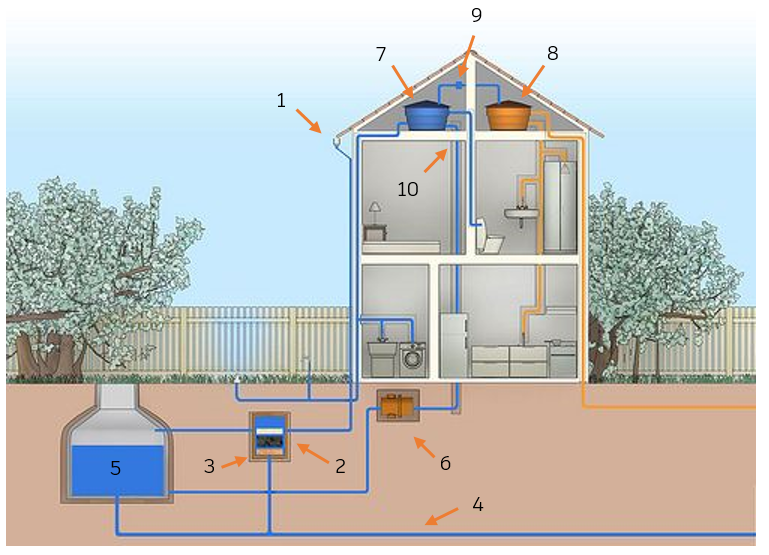
\includegraphics[width=0.6\textwidth]{figuras/esquema_cisterna.png}
    \caption*{\tiny{Fonte: Adaptado (ECOMONTES, 2016)}}
    \label{fig:esquema_cisterna}
  \end{figure}

\end{frame}

\begin{frame}{Metodologia}{Análise e definição das características do projeto}
 
  \begin{table}[]
    \hspace*{-3cm}
    \begin{centering}
    \resizebox{0.55\textwidth}{!}{\begin{minipage}{\textwidth}
    \begin{tabular}{c|c|c}
      \hline
      \textbf{Identificador} & \textbf{Elemento} & \textbf{Descrição} \\ \hline
      1 & Calha coletora & \begin{tabular}[c]{@{}c@{}}Elemento convencional para coleta e \\ descarte de água da chuva\end{tabular} \\ \hline
      2 & Filtro A (cascalho fino) & \begin{tabular}[c]{@{}c@{}}Elemento para realização de \\ filtragem de pequenas impurezas\end{tabular} \\ \hline
      3 & Filtro B (cascalho grosso) & \begin{tabular}[c]{@{}c@{}}Elemento para realização de \\ filtragem de impurezas\end{tabular} \\ \hline
      4 & Tubulação de descarte & \begin{tabular}[c]{@{}c@{}}Tubulação utilizada como rota de escoamento \\ quando o reservatório não está em uso ou \\ está cheio\end{tabular} \\ \hline
      5 & Reservatório de coleta & Cisterna propriamente dita \\ \hline
      6 & Motobomba ou bomda d'água & \begin{tabular}[c]{@{}c@{}}Elemento utilizado para realização do \\ ganho de elevação da água\end{tabular} \\ \hline
      7 & Caixa d'água auxiliar & \begin{tabular}[c]{@{}c@{}}Caixa d'água convencional com alimentação \\ oriunda da bomba d'água\end{tabular} \\ \hline
      8 & Caixa d'água convencional & \begin{tabular}[c]{@{}c@{}}Caixa d'água padrão com alimentação \\ da estação de água da cidade\end{tabular} \\ \hline
      9 & Elo de ligação & \begin{tabular}[c]{@{}c@{}}Ligação utilizada para abastecer a caixa d'água \\ auxiliar quando a cisterna está seca \\ ou em manutenção\end{tabular} \\ \hline
      10 & Distribuidor & \begin{tabular}[c]{@{}c@{}}Elementos de distribuição de água \\ para pontos estratégicos\end{tabular} \\ \hline
    \end{tabular}
    \caption{Identificação dos elementos da Figura \autoref{fig:esquema_cisterna}.}
  \end{minipage}}
  \end{centering}
  \end{table}

\end{frame}

\begin{frame}{}

  \begin{figure}[H]
    \vspace*{-0.3cm}
    \centering
    \caption{Esquema básico do projeto.}
    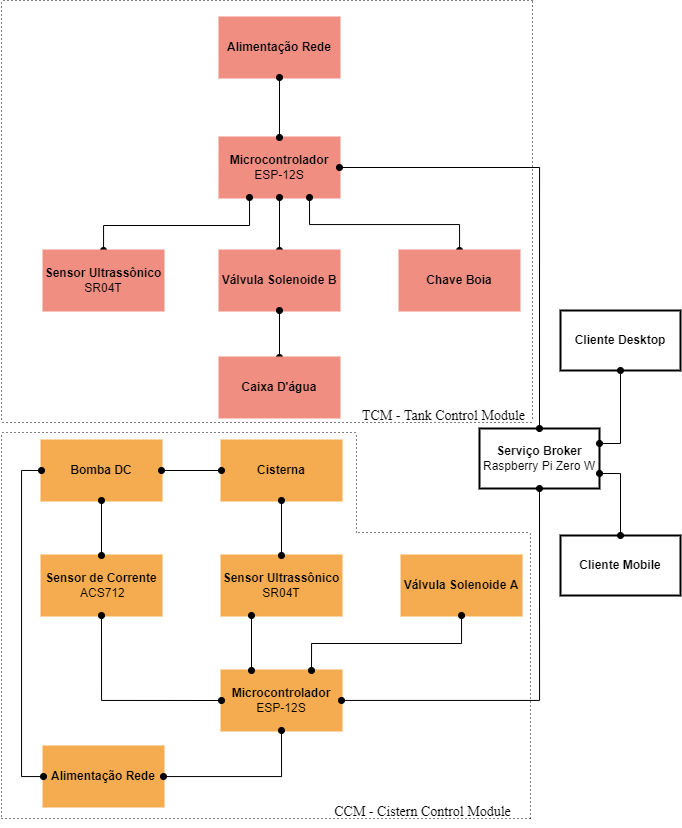
\includegraphics[width=0.5\textwidth]{figuras/esquema_basico_proj_2.png}
    \caption*{\tiny{Fonte: Própria}}
    \label{fig:esquema_proj}
    
  \end{figure}

  
\end{frame}

\begin{frame}{Metodologia}{Análise e definição das características do projeto}
 \begin{itemize}
   \item Outro ponto importante desta parte do projeto foi estabelecer as medidas de volume da cisterna e da caixa d'água assim como as equações de volume tendo como variável a altura do líquido.
 \end{itemize}

\end{frame}

\begin{frame}{}
  \begin{figure}[H]
    \centering
    \caption{Representação das dimensões da cisterna.}
    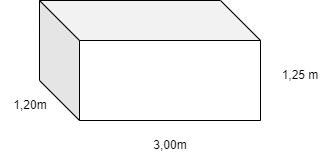
\includegraphics[width=0.3\textwidth]{figuras/volume.png}
    \caption{\tiny{Fonte: Própria}}
    \label{fig:volume_cisterna}
  \end{figure}
  
  Equação de volume associada:
  
  \begin{equation}
  V = c \cdot l \cdot (h-s)  
  \end{equation}
  
  \begin{itemize}
    \item $V$ é o volume;
    \item $h$ é a altura do tanque;
    \item $s$ é a leitura de distância do sensor;
    \item $c$ é o comprimento do tanque;
    \item $l$ é o largura do tanque.
  \end{itemize}
\end{frame}

\begin{frame}{}
  \vspace*{-0.1cm}
  \begin{figure}[H]
    \centering
    \caption{Representação das dimensões da caixa d'água (valores em centímetros).}
    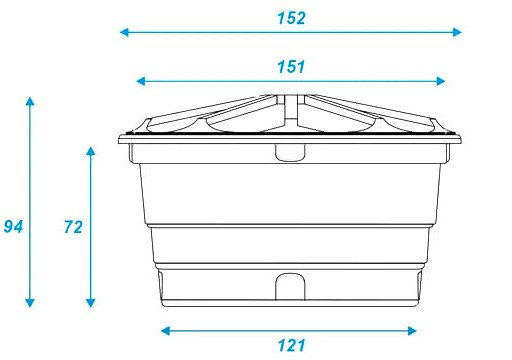
\includegraphics[width=0.3\textwidth]{figuras/caixa.jpg}
    \caption*{\tiny{tendtudo.com, 2021}}
    \label{fig:volume_tanque}
  \end{figure}
  
  Equação de volume associada:
  
  \begin{equation}
  V = \frac{\pi\cdot (h-s)\cdot (R^{2}+R\cdot r+r^{2})}{3} 
  \end{equation}
  
  \begin{itemize}
    \item $V$ é o volume;
    \item $h$ é a altura do tanque;
    \item $s$ é a leitura de distância do sensor;
    \item $R$ é o raio maior;
    \item $r$ é o raio menor.
  \end{itemize}
\end{frame}

\begin{frame}{Desenvolvimento dos elementos de \textit{Hardware}}
  \begin{itemize}
    \item Nesse momento foram definidos todos os elementos de \textit{hardware} necessários para o desenvolvimento do trabalho: dispositivos eletrônicos, documentos como \textit{Datasheets}, catálogos e informativos de dispositivos elétricos.
  \end{itemize}
  
\end{frame}

\begin{frame}{Desenvolvimento dos elementos de \textit{Hardware}}{O circuito de alimentação}
  \begin{figure}[H]
    \centering
    \caption{Esquma de ligação do circuito de alimentação}
    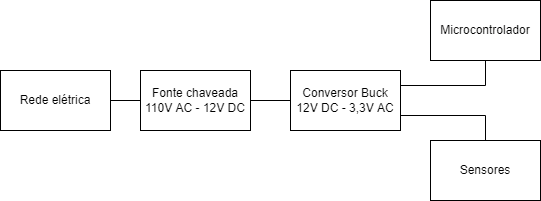
\includegraphics[width=0.6\textwidth]{figuras/alimentacao.png}
    \caption*{\tiny{Fonte: Própria.}}
    \label{fig:alimentacao_esquema}
  \end{figure}
\end{frame}



\begin{frame}{Desenvolvimento dos elementos de \textit{Hardware}}{O circuito de alimentação}
  \begin{figure}[H]
    \centering
    \caption{Aplicação típica do LM2596.}
    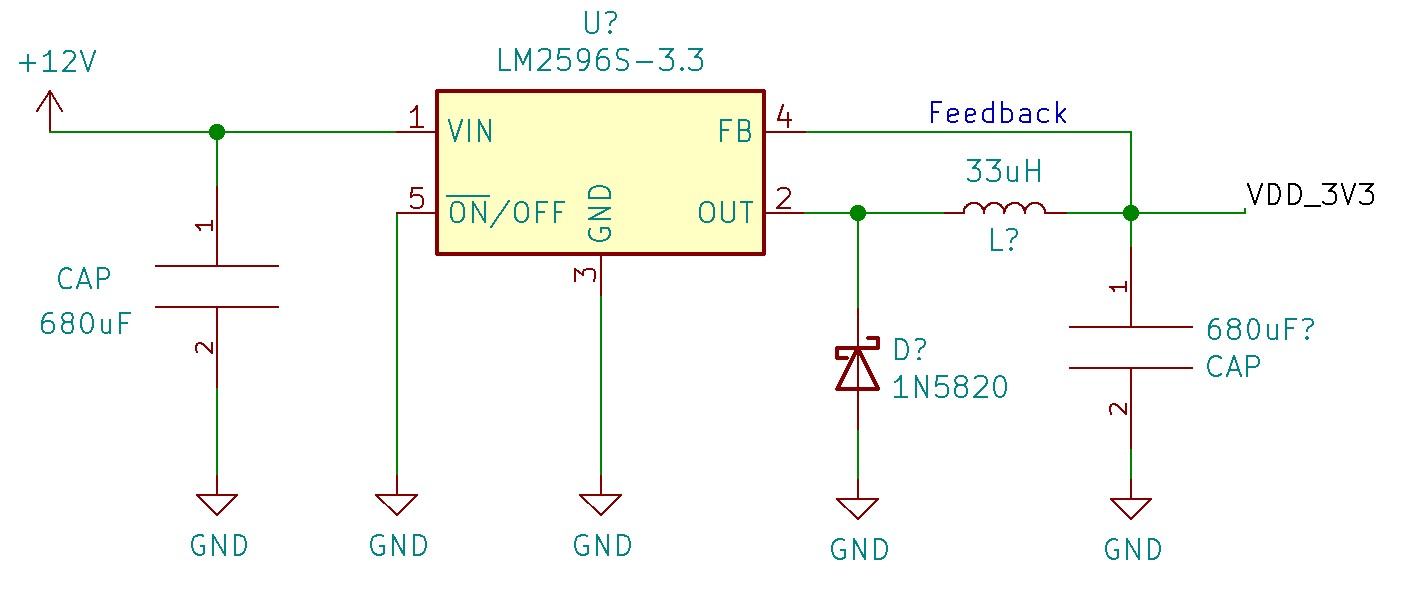
\includegraphics[width=0.7\textwidth]{figuras/conversor_buck.jpg}
    \caption*{\tiny{Fonte: Própria.}}
    \label{fig:conversor_buck}
  \end{figure}
\end{frame}

\begin{frame}{Desenvolvimento dos elementos de \textit{Hardware}}{O circuito de alimentação}
  \begin{figure}[H]
    \centering
    \caption{Teste em bancada do módulo com LM2596.}
    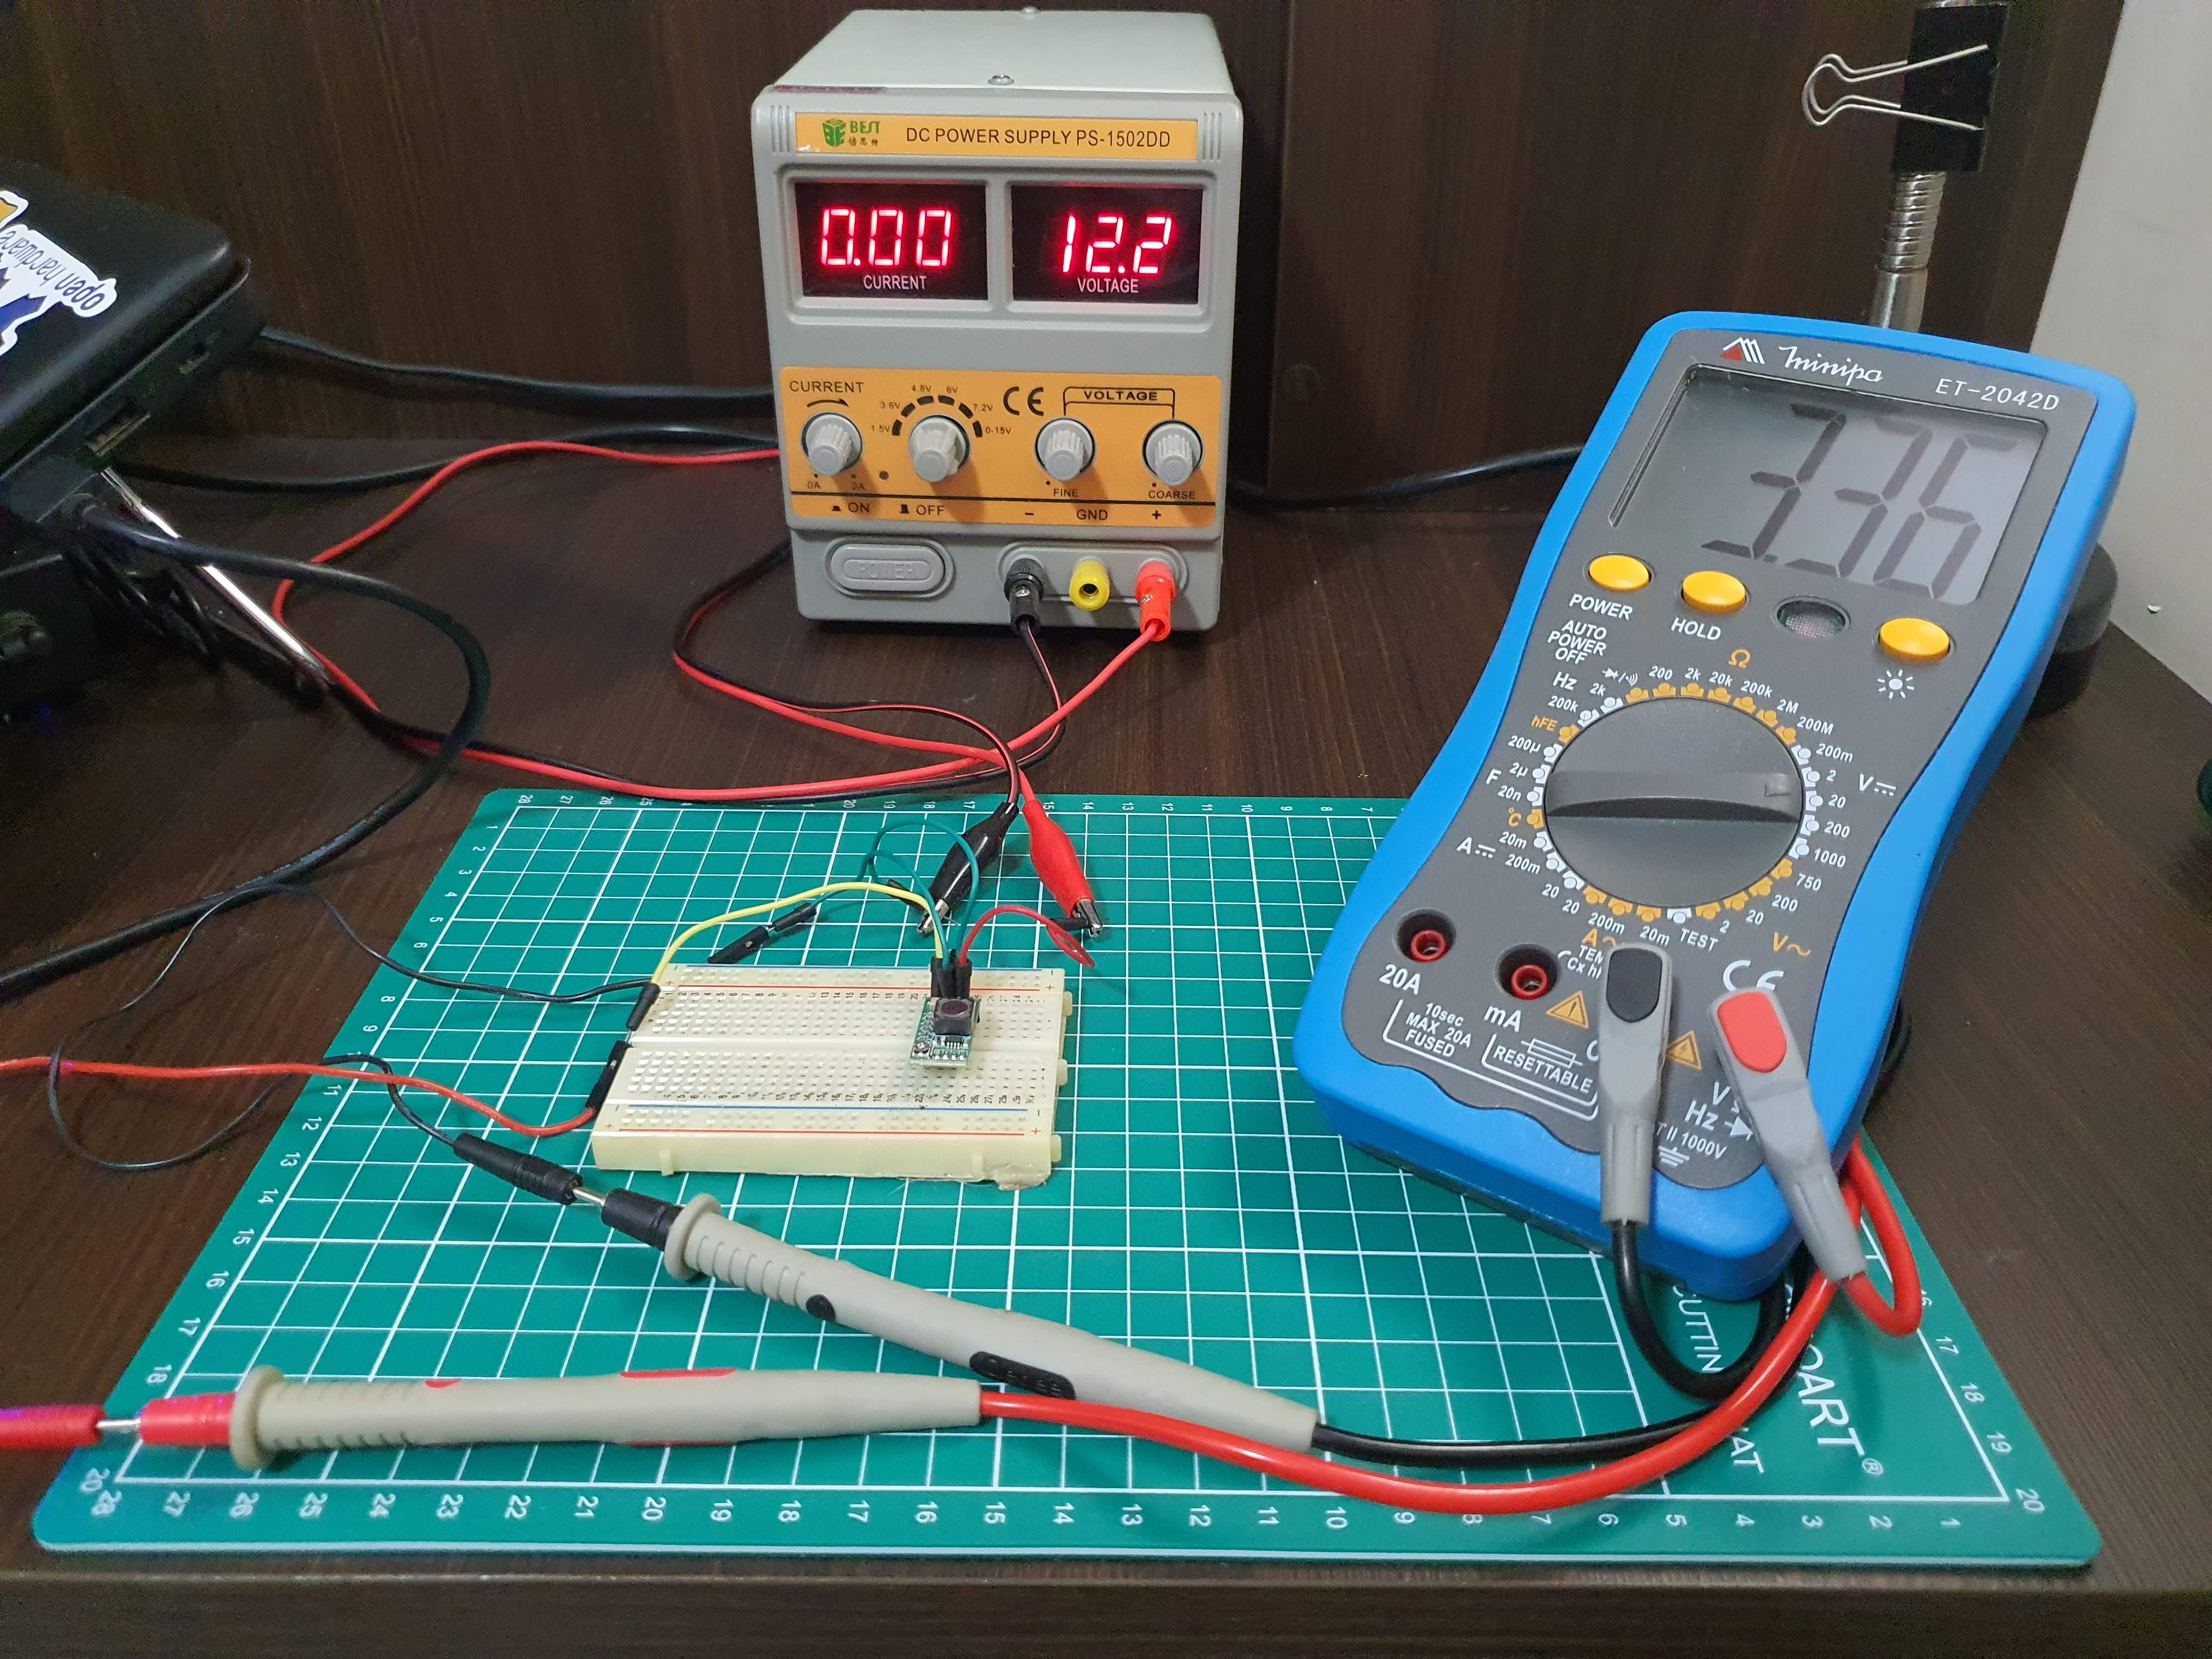
\includegraphics[width=0.4\textwidth]{figuras/conversor_buck_teste.jpg}
    \caption*{\tiny{Fonte: Própria.}}
    \label{fig:conversor_buck_teste}
  \end{figure}
\end{frame}

\begin{frame}{Desenvolvimento dos elementos de \textit{Hardware}}{O circuito de detecção de fechadura da chave}
  \begin{figure}[H]
    \centering
    \caption{Esquema de aplicação da chave boia}
    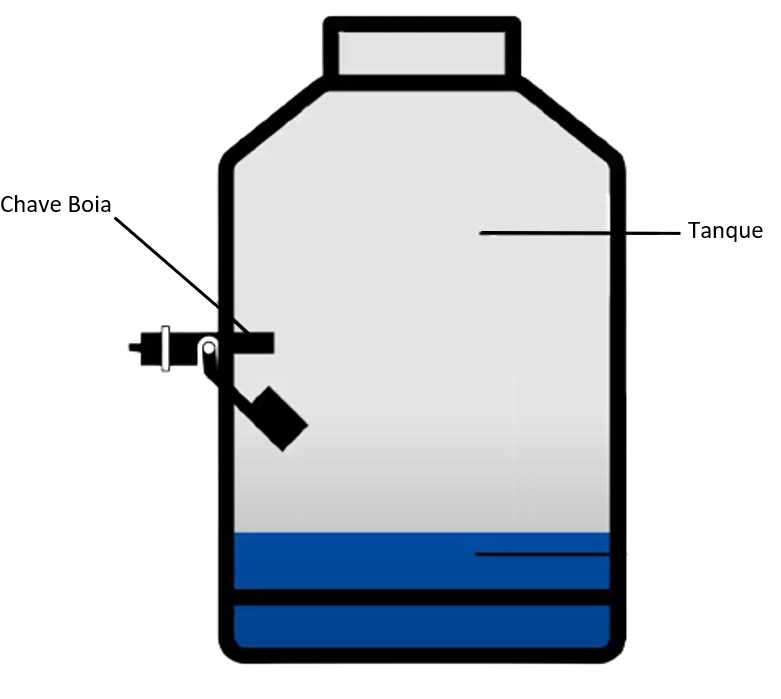
\includegraphics[width=0.3\textwidth]{figuras/chave_boia_aplicacao.png}
    \caption*{\tiny{Fonte: Própria.}}
    \label{fig:chave_boia_aplicacao}
  \end{figure}
\end{frame}

\begin{frame}{Desenvolvimento dos elementos de \textit{Hardware}}{O circuito de detecção de fechadura da chave}
  \begin{itemize}
    \item Para executar a detecção com essa chave de dois estados foi-se necessário aplicar um circuito com resistores de \textit{pullup} (\autoref{fig:chave_boia_pullup}).
  \end{itemize}

\begin{figure}[H]
	\centering
	\caption{Esquema de ligação elétrica da chave boia.}
	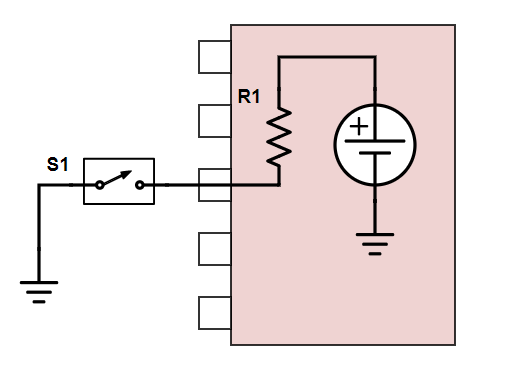
\includegraphics[width=0.3\textwidth]{figuras/pullup.png}
	\caption*{\tiny{Fonte: Própria.}}
	\label{fig:chave_boia_pullup}
\end{figure}
\end{frame}

\begin{frame}{Desenvolvimento dos elementos de \textit{Hardware}}{O circuito de detecção de fechadura da chave}
  \begin{figure}[H]
    \centering
    \caption{Chave boia acoplada ao ESP-12S através de um pino digital com \textit{INPUT PULLUP}.}
    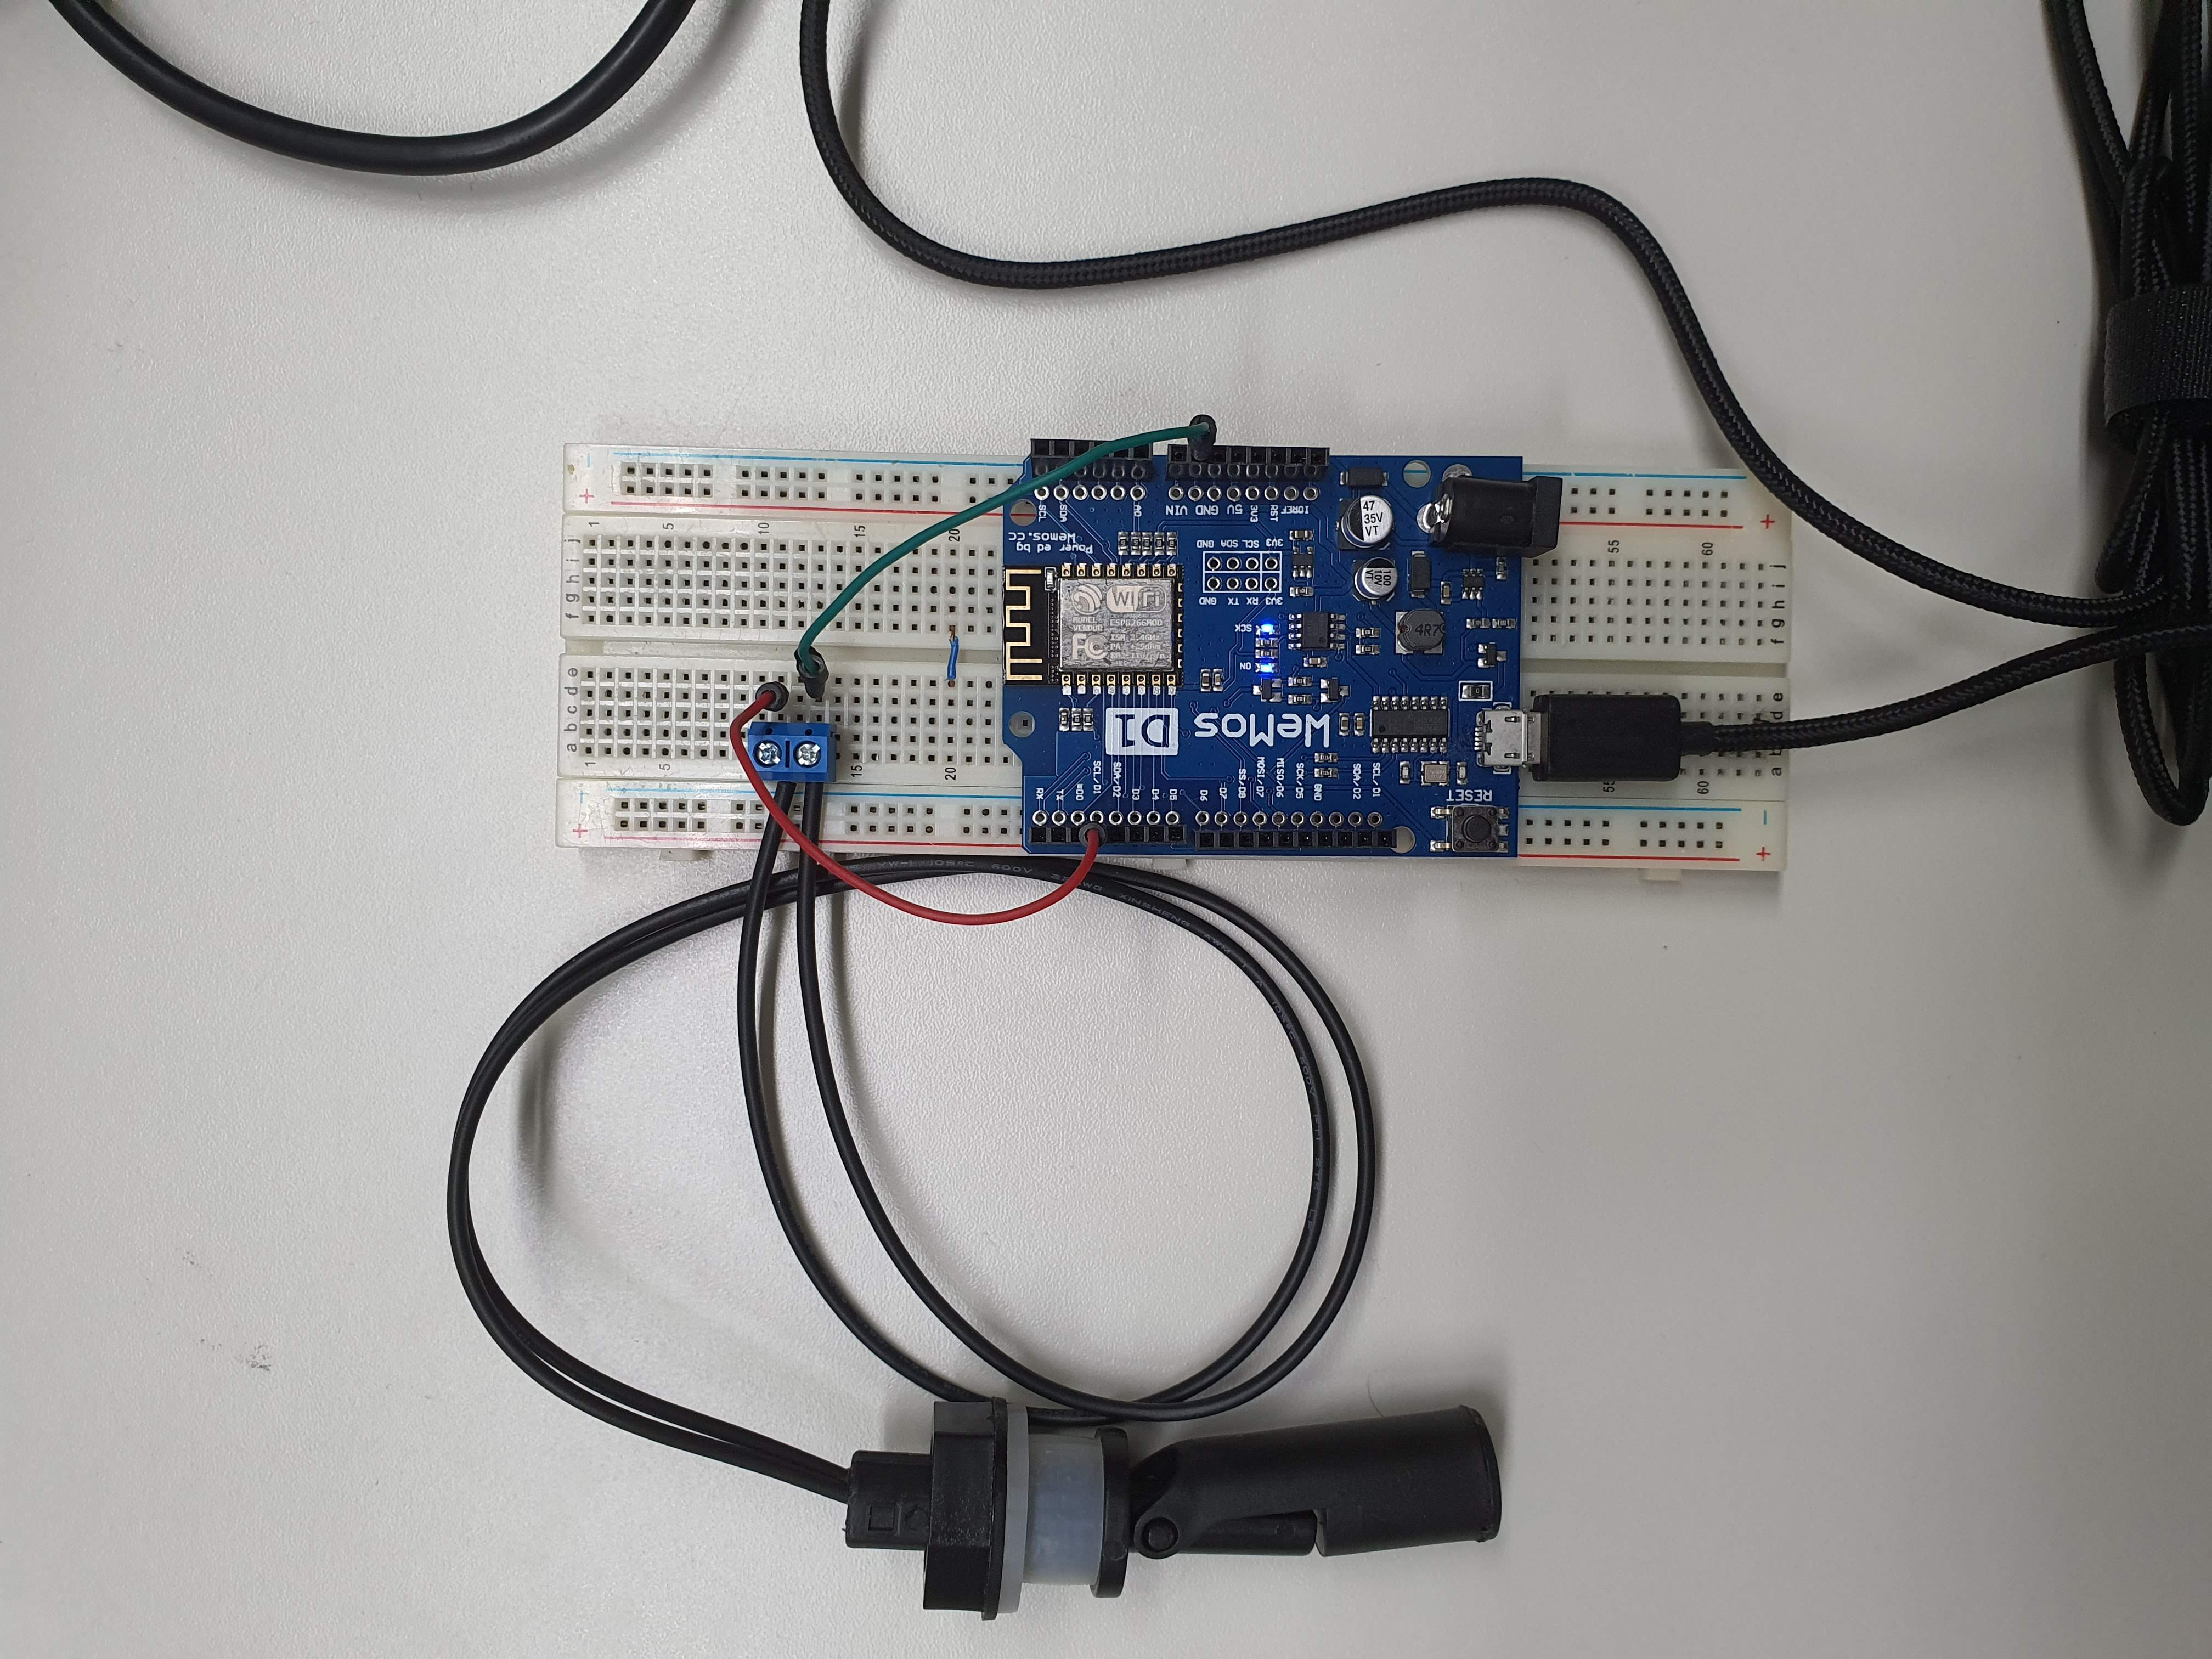
\includegraphics[width=0.5\textwidth]{figuras/teste_chave_boia.jpg}
    \caption*{\tiny{Fonte: Própria.}}
    \label{fig:chave_boia_pullup_teste}
  \end{figure}
  
\end{frame}

\begin{frame}{Desenvolvimento dos elementos de \textit{Hardware}}{O circuito de medição de nível}
  \begin{figure}[H]
    \centering
    \caption{Teste de ligação sensor do módulo JSN-SR04T.}
    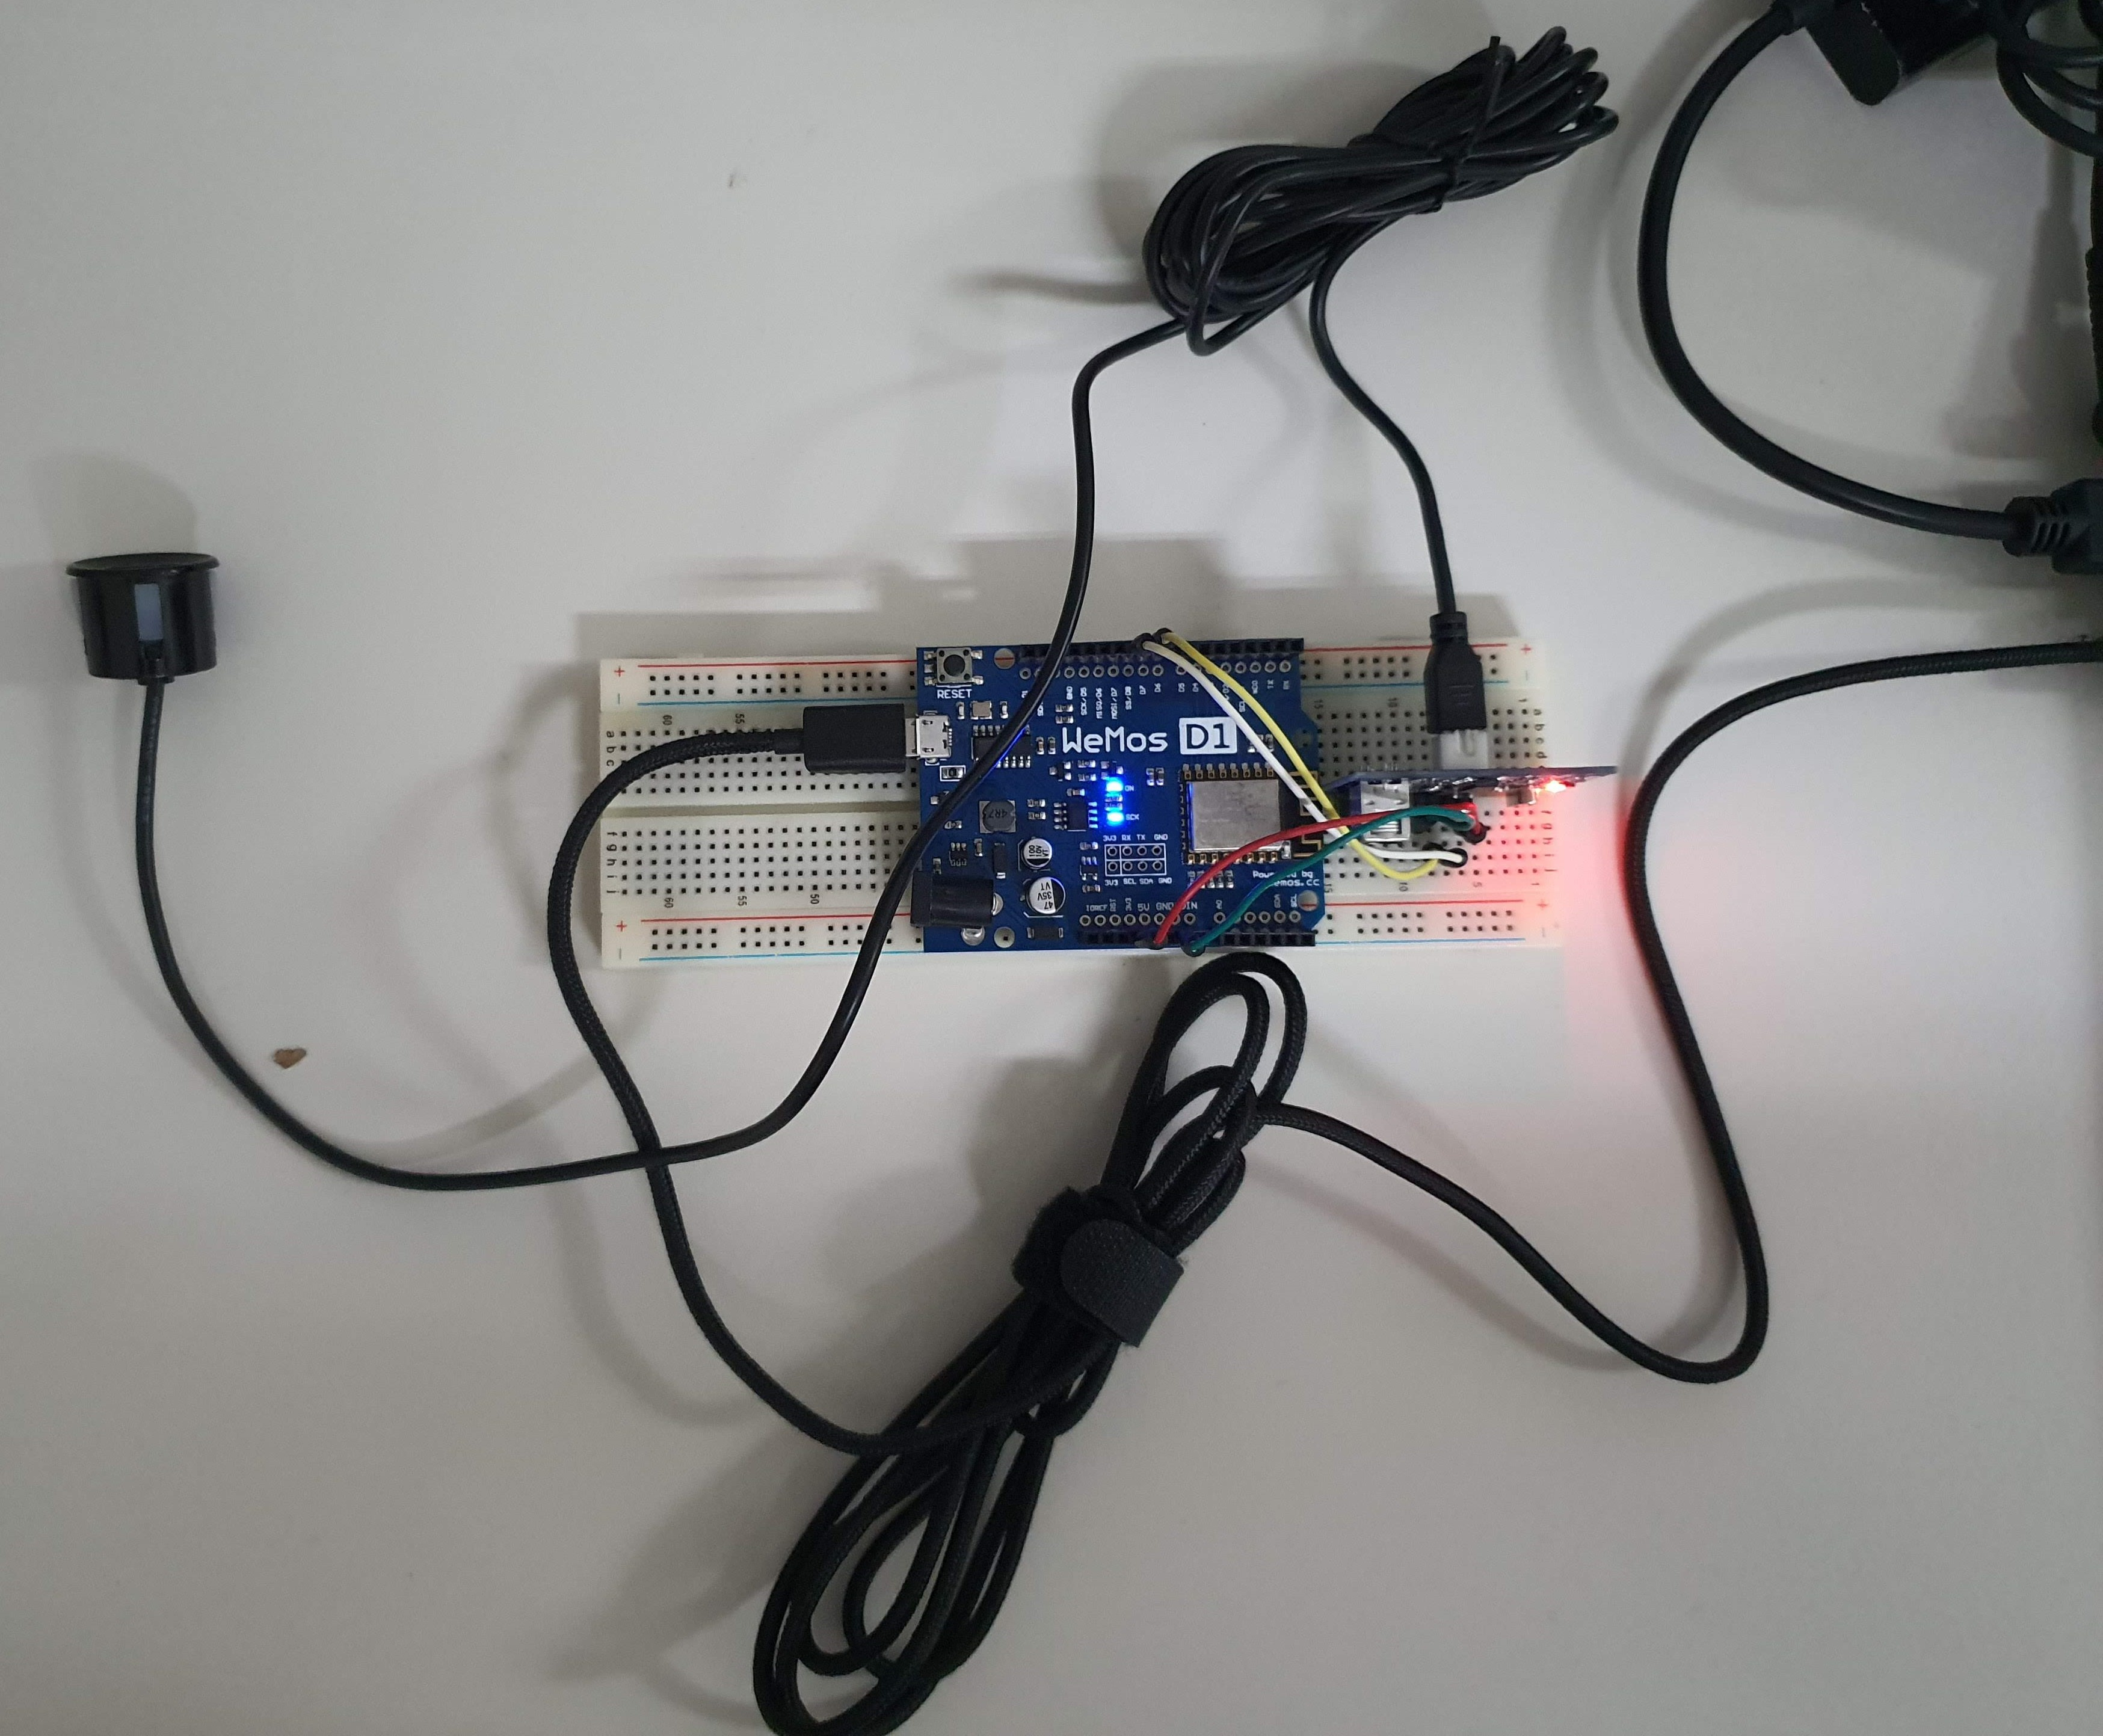
\includegraphics[width=0.4\textwidth]{figuras/teste_ultrassonico.jpg}
    \caption*{\tiny{Fonte: Própria.}}
    \label{fig:sensor_ultrassonico}
  \end{figure}
  
\end{frame}

\begin{frame}{Desenvolvimento dos elementos de \textit{Hardware}}{O circuito de medição de nível}
  \begin{figure}[H]
    \centering
    \caption{Potenciômetro soldado ao módulo.}
    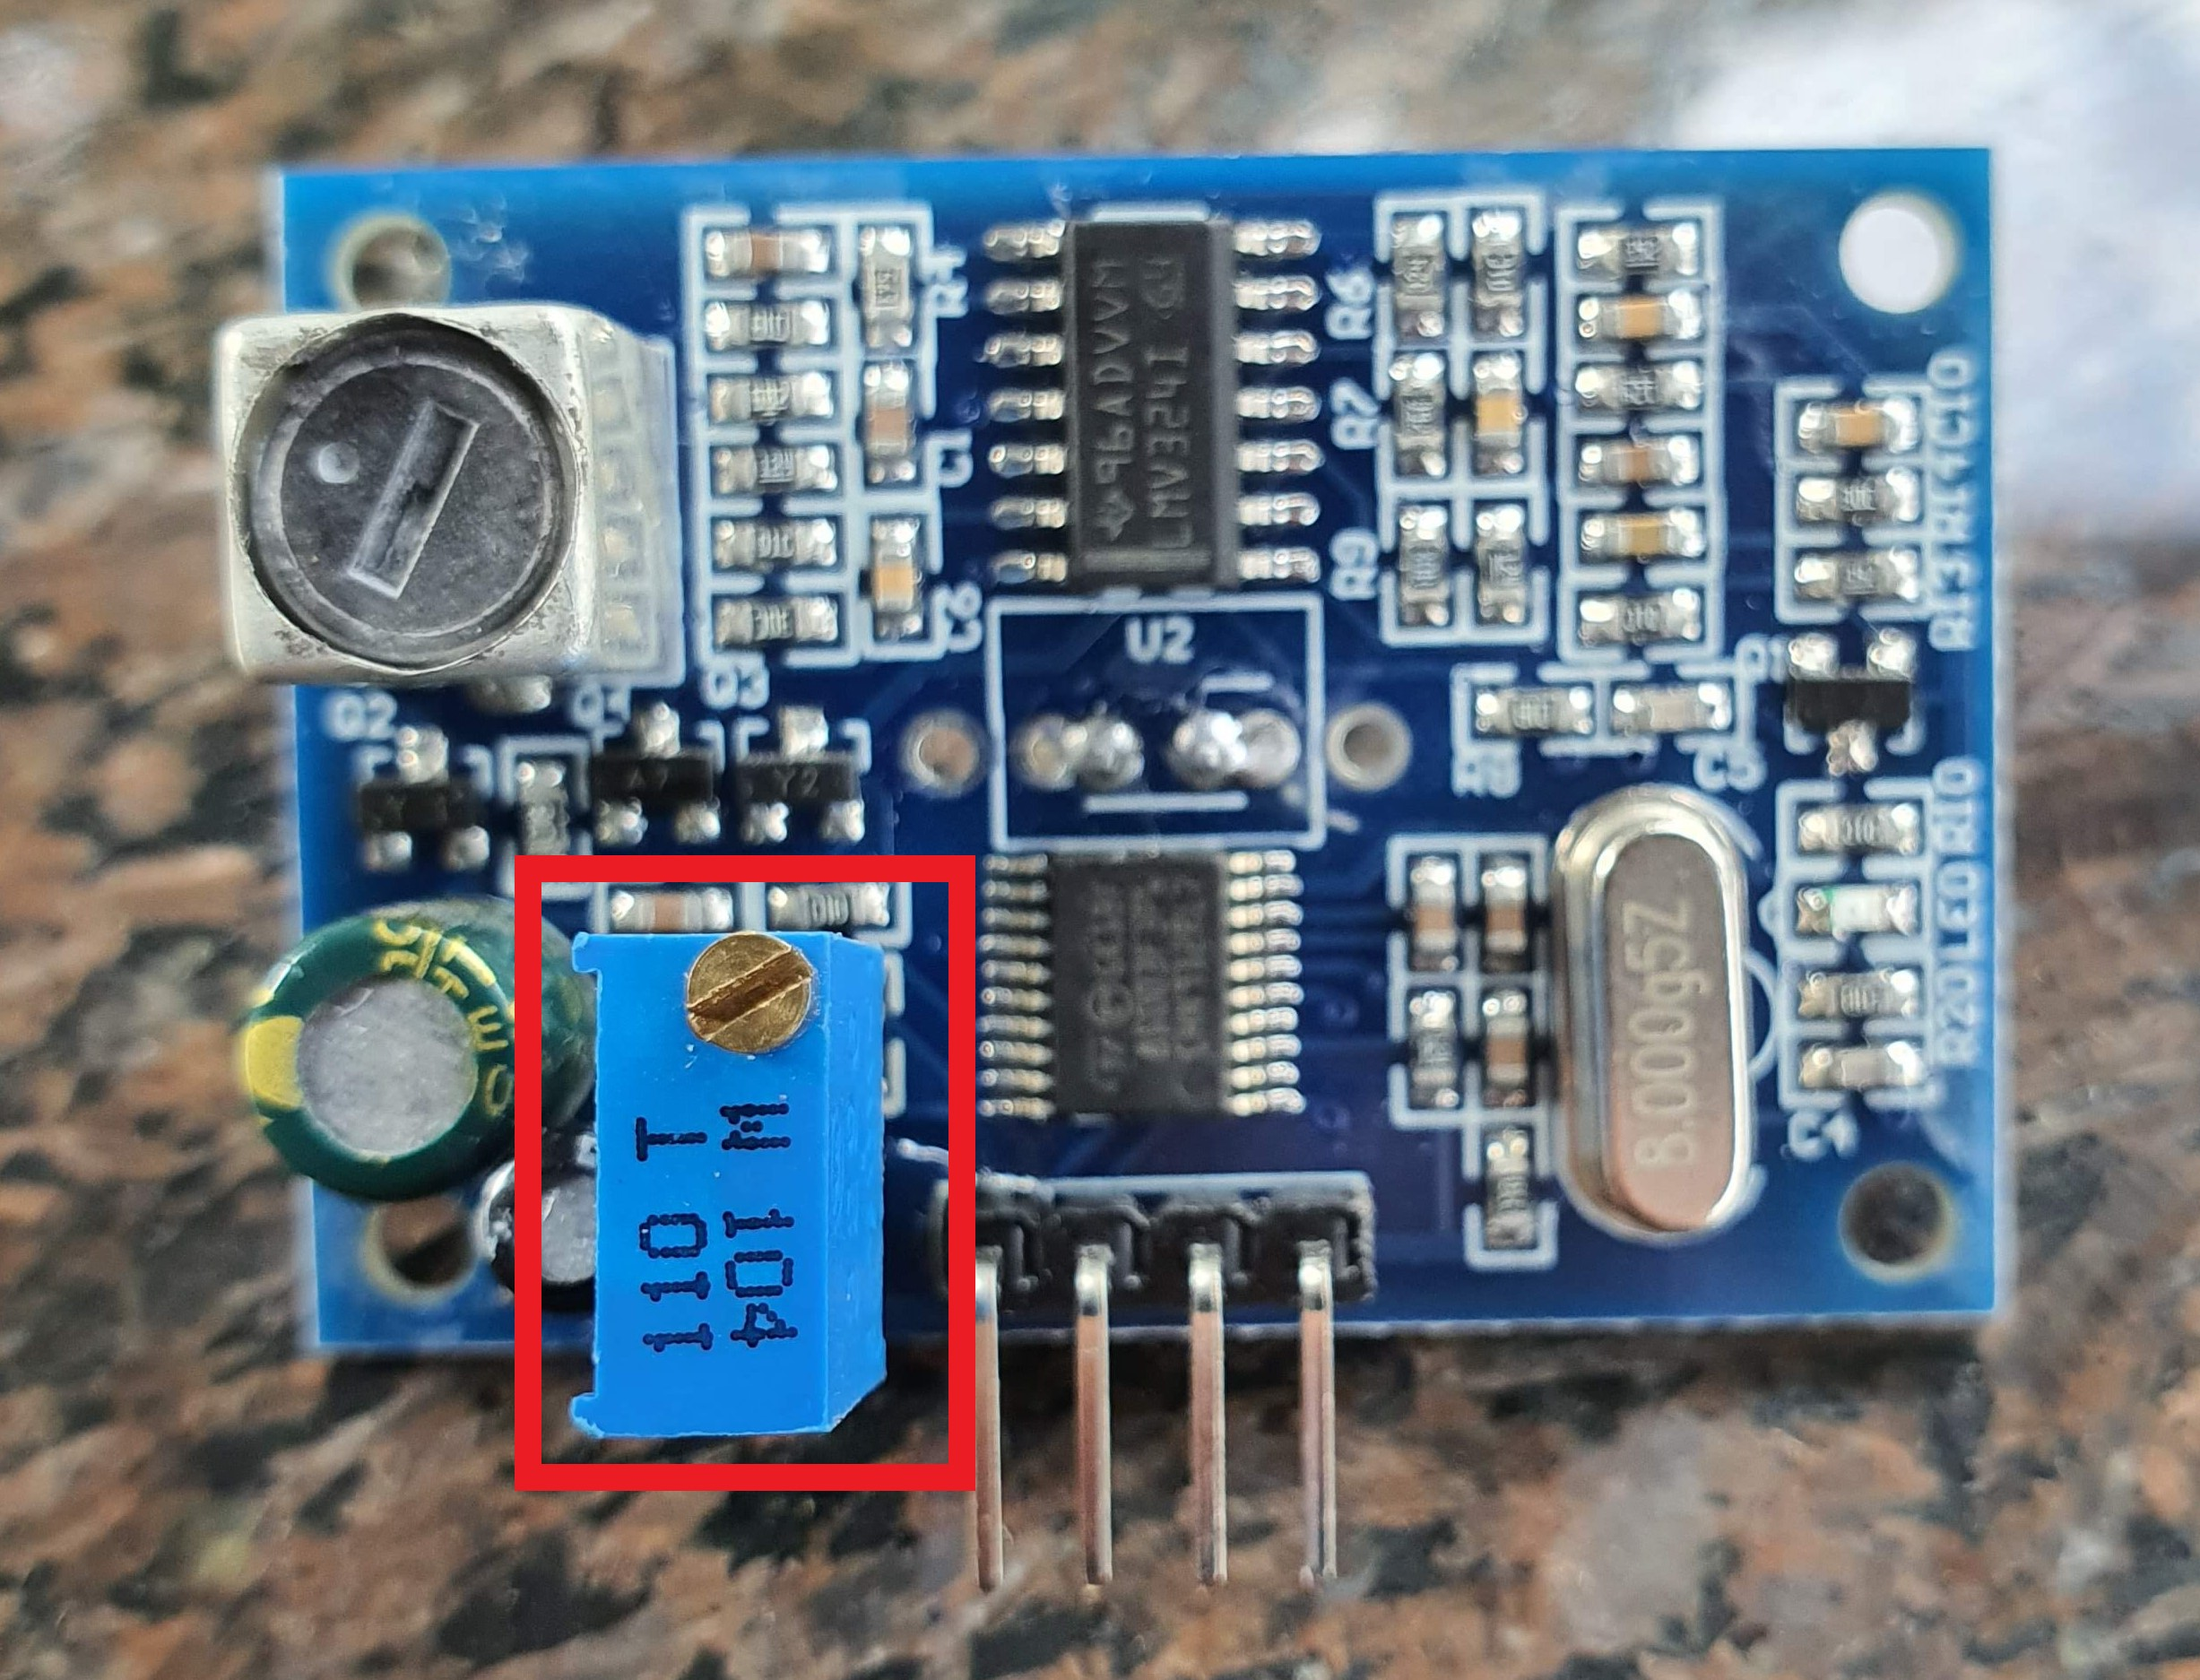
\includegraphics[width=0.4\textwidth]{figuras/ultrassonico_res.jpg}
    \caption*{\tiny{Fonte: Própria.}}
    \label{fig:ultrasonico_res}
  \end{figure}
  
\end{frame}

\begin{frame}{Desenvolvimento dos elementos de \textit{Hardware}}{O circuito de ativação da motobomba}
  \begin{figure}[H]
    \centering
    \caption{Diagrama de ativação do motor}
    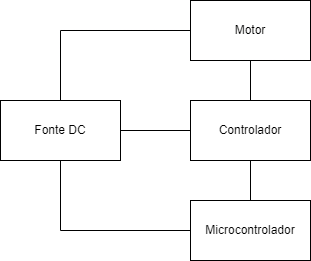
\includegraphics[width=0.4\textwidth]{figuras/ativacao_motor.png}
    \caption*{\tiny{Fonte: Própria.}}
    \label{fig:diagrama_ativacao_motor}
  \end{figure}
\end{frame}

\begin{frame}{Desenvolvimento dos elementos de \textit{Hardware}}{O circuito de ativação da motobomba}
  \begin{figure}[H]
    \centering
    \caption{Teste da motobomba}
    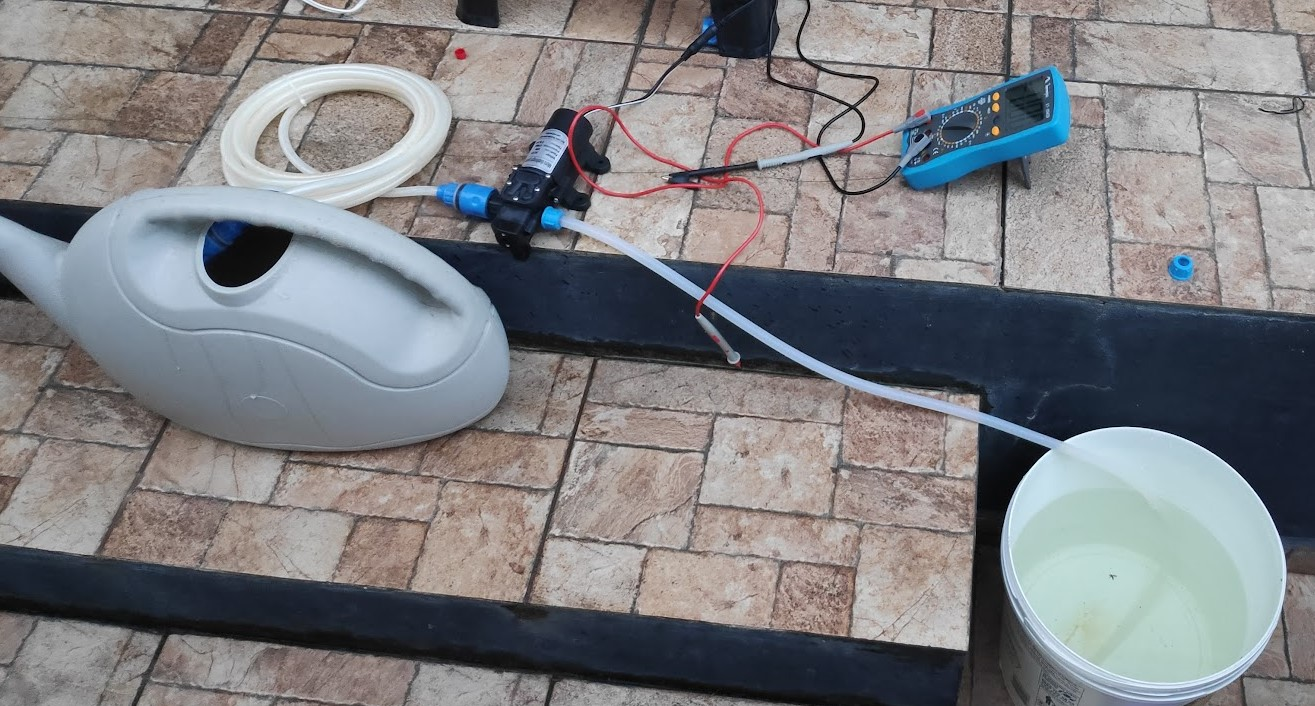
\includegraphics[width=0.6\textwidth]{figuras/teste_motor.jpg}
    \caption*{\tiny{Fonte: Própria.}}
    \label{fig:teste_ativacao_motor}
  \end{figure}
\end{frame}

\begin{frame}{Desenvolvimento dos elementos de \textit{Hardware}}{O circuito de ativação da motobomba}
  \begin{itemize}
    \item Com os dados obtidos através dos testes, deu-se início a procura de componentes e metodologias para o controle \textit{ON-OFF} de motores de corrente contínua;
    \item Como o microcontrolador não possui tesão nem corrente suficientes para ativar o motor, foi-se necessário desenvolver uma ativação indireta transistorizada;
  \end{itemize}

\end{frame}

\begin{frame}{Desenvolvimento dos elementos de \textit{Hardware}}{O circuito de ativação da motobomba}
  \begin{figure}[H]
    \centering
    \caption{Diagrama de ativação com partida lenta}
    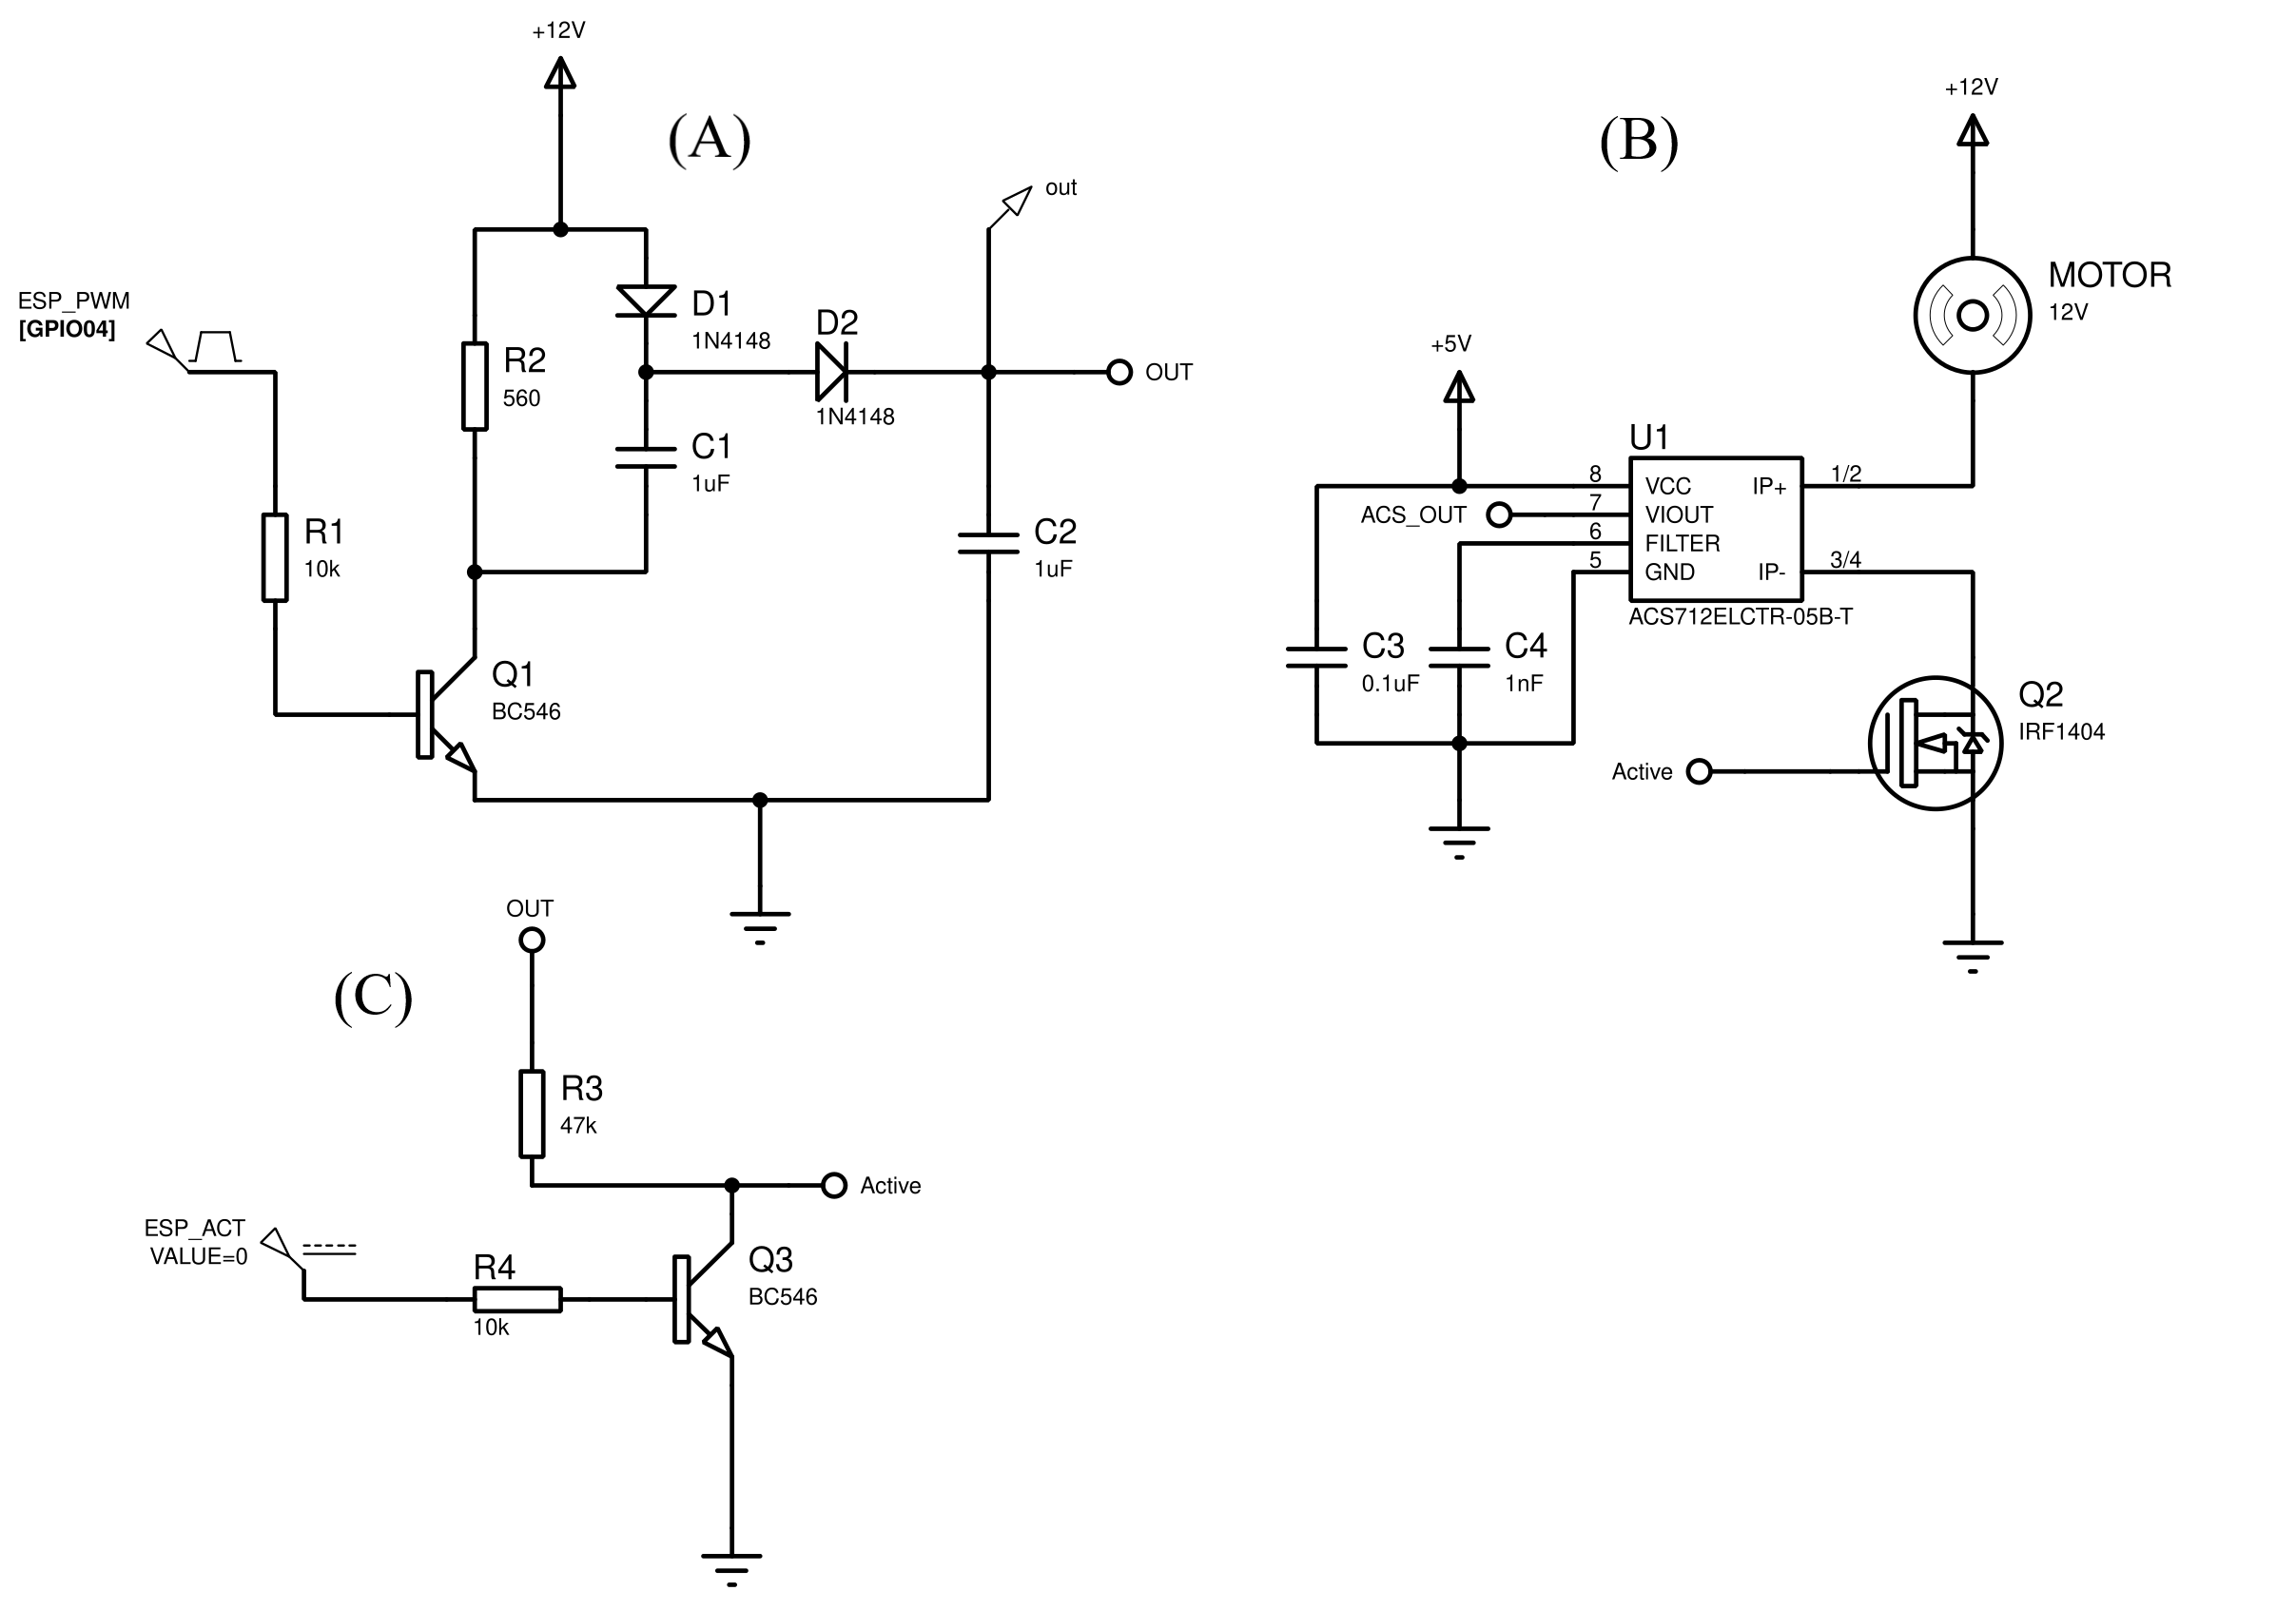
\includegraphics[width=0.7\textwidth]{figuras/diagrama_ativação_bomba.png}
    \caption*{\tiny{Fonte: Própria.}}
  \end{figure} 
\end{frame}

\begin{frame}{Desenvolvimento dos elementos de \textit{Hardware}}{O circuito de ativação da motobomba}
  \begin{figure}[H]
    \centering
    \caption{Resultados obtidos da leitura de pontos estratégicos do dobrador de tensão montado}
    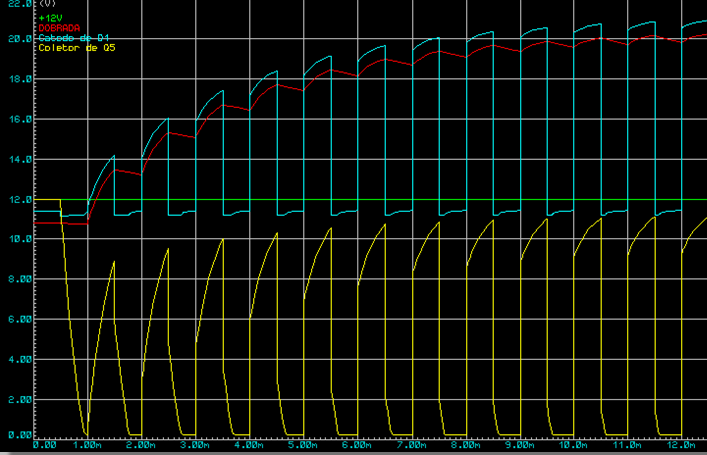
\includegraphics[width=0.7\textwidth]{figuras/dobrador.png}
    \caption*{\tiny{Fonte: Própria.}}
  \end{figure}
\end{frame}

\begin{frame}{Desenvolvimento dos elementos de \textit{Hardware}}{O circuito de ativação da motobomba}
  \begin{figure}[H]
    \centering
    \caption{Circuito do dobrador de tensão montado.}
    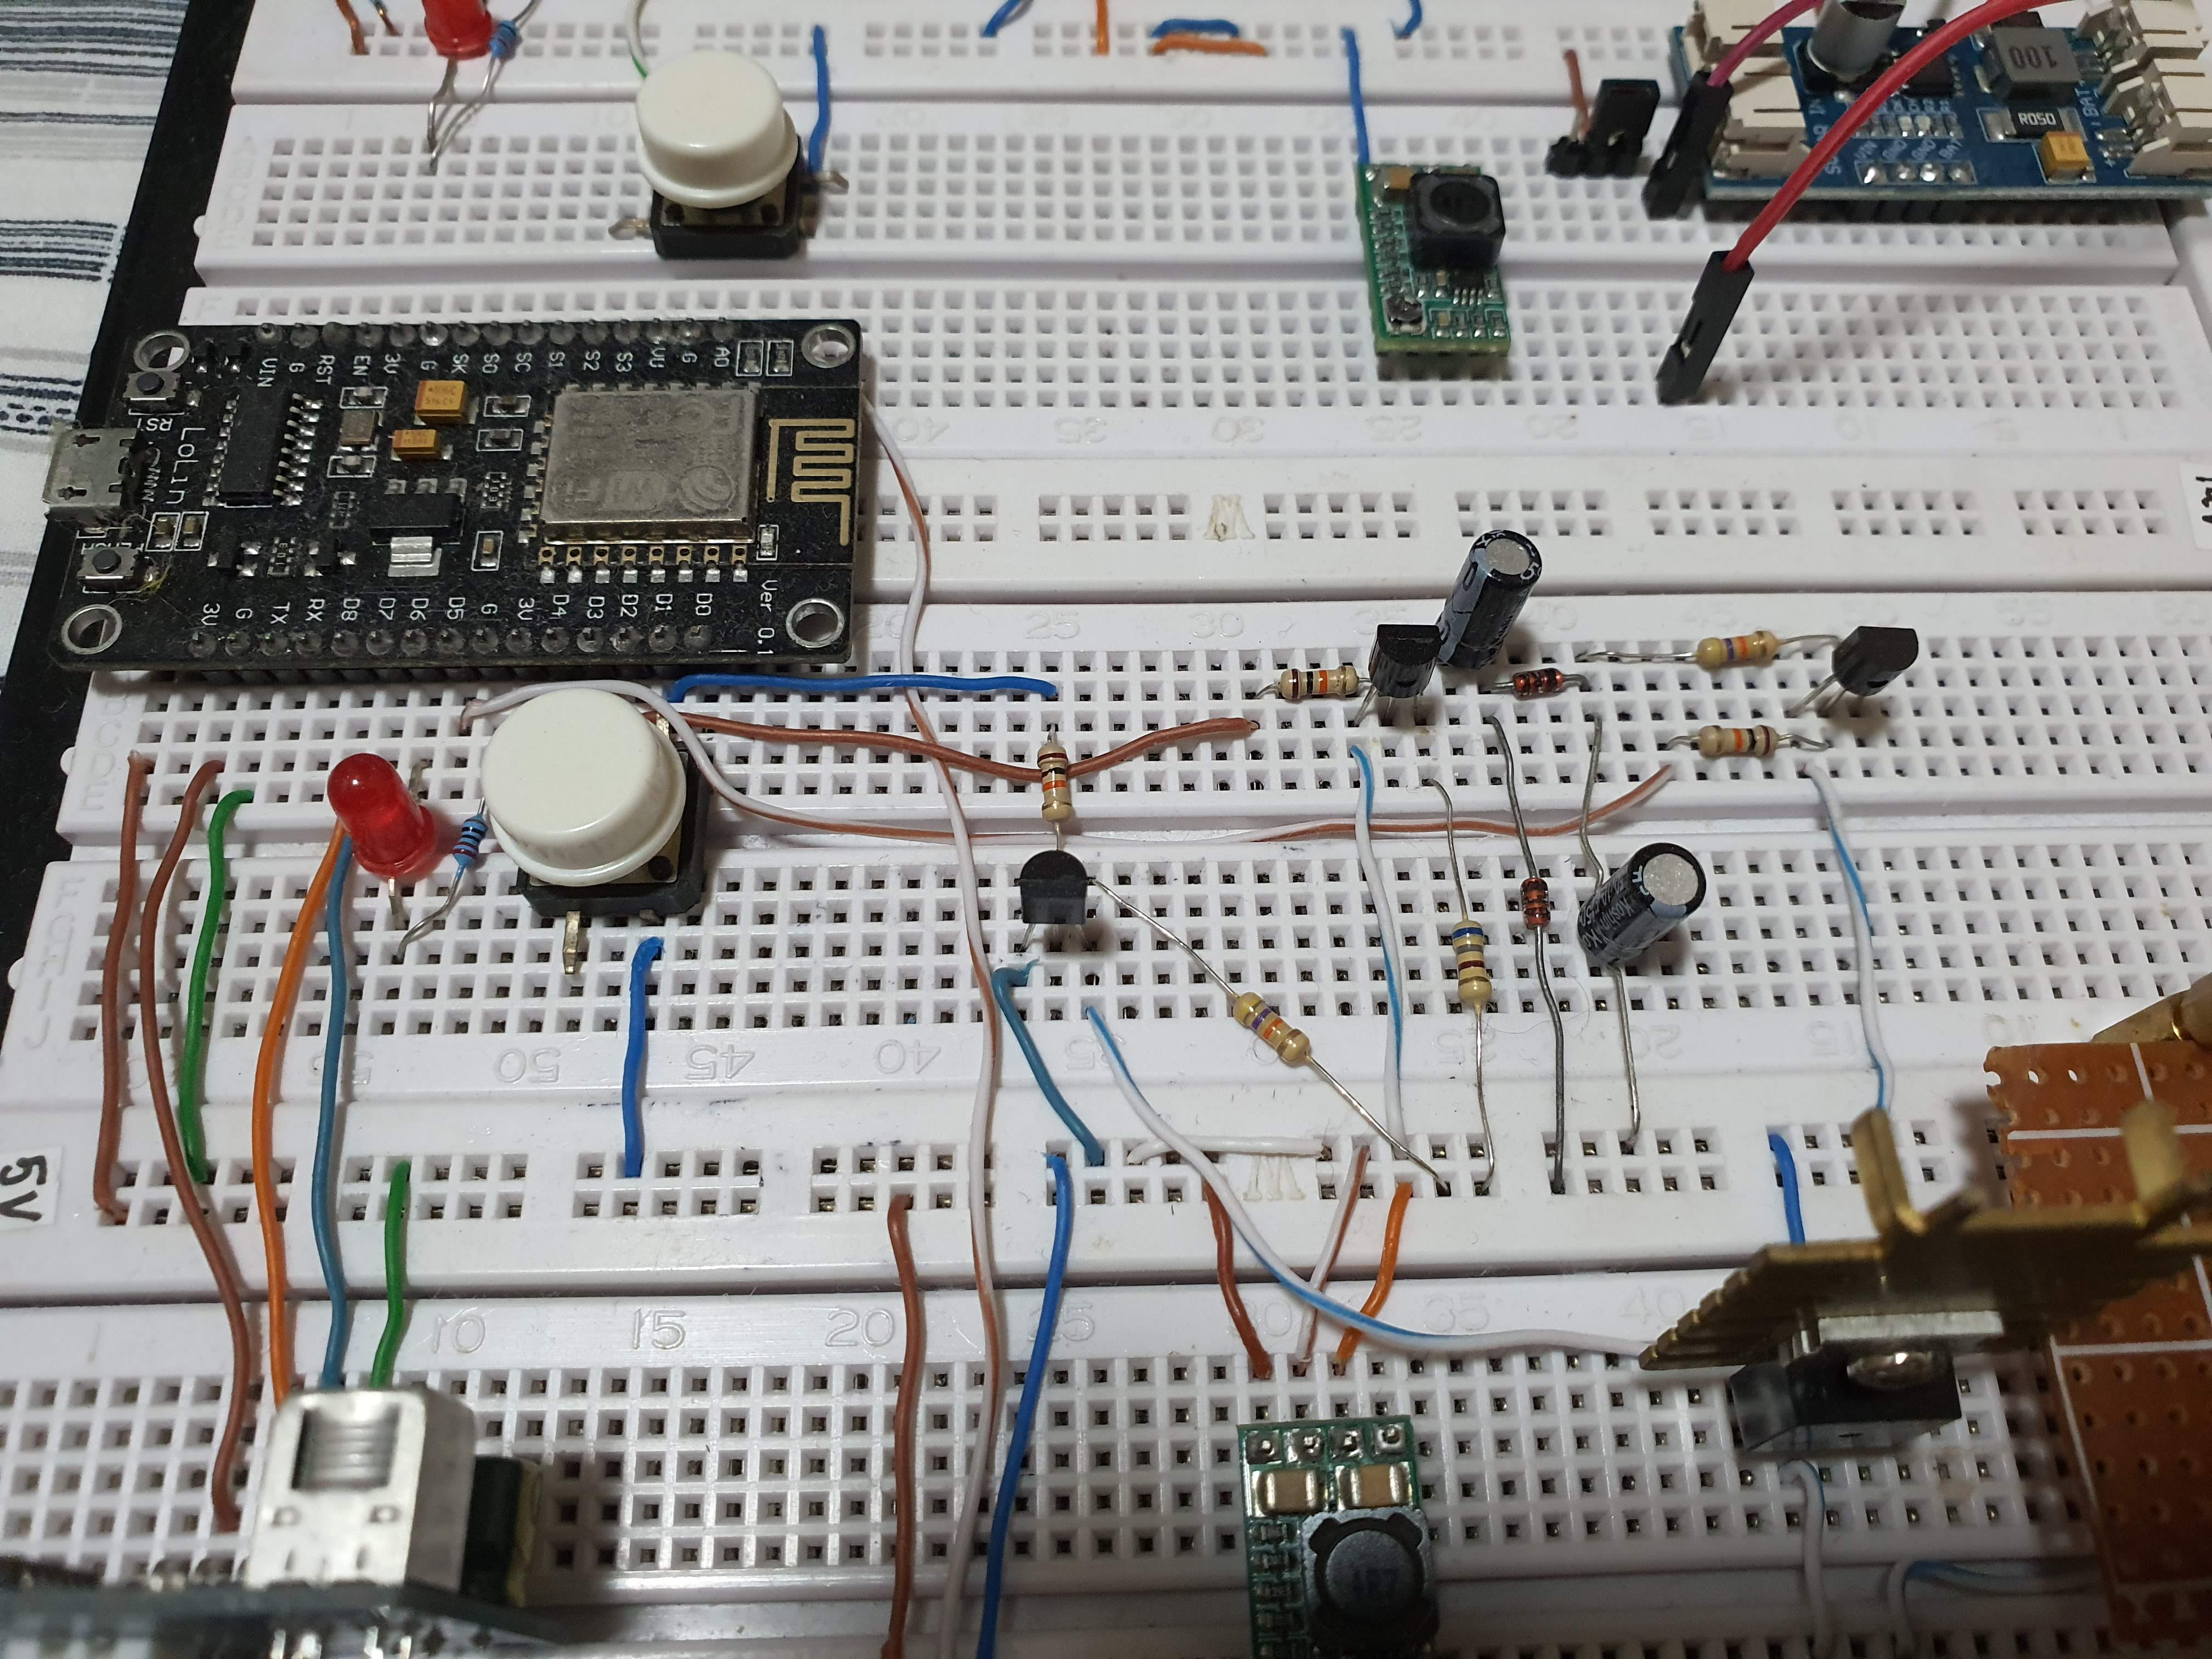
\includegraphics[width=0.5\textwidth]{figuras/dobrador_montado.jpg}
    \caption*{\tiny{Fonte: Própria.}}
    \label{fig:dobrador_montado}
  \end{figure} 
  
\end{frame}

\begin{frame}{Desenvolvimento dos elementos de \textit{Hardware}}{O circuito de ativação da motobomba}
  \begin{figure}[H]
    \centering
    \caption{Placa com Transistor IRF1404.}
    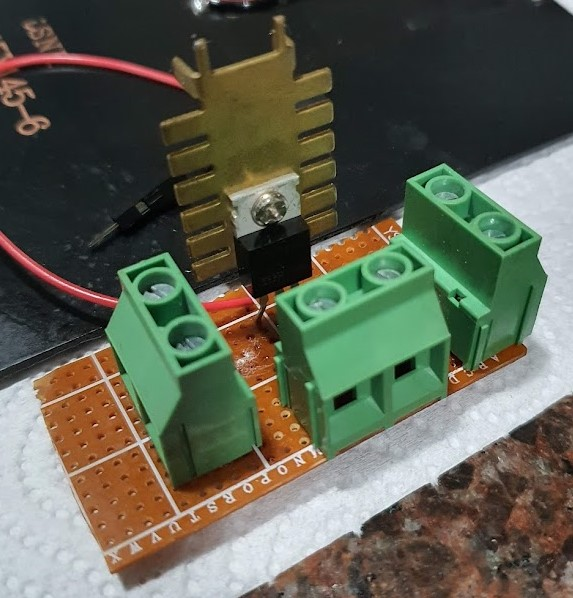
\includegraphics[width=0.3\textwidth]{figuras/transistor_motor.jpg}
    \caption*{\tiny{Fonte: Própria.}}
    \label{fig:dobrador_montado}
  \end{figure} 
  
\end{frame}

\begin{frame}{Desenvolvimento dos elementos de \textit{Hardware}}{O circuito de ativação da válvula}
  \begin{figure}[H]
    \centering
    \caption{Diagrama de ativação da válvula solenoide.}
    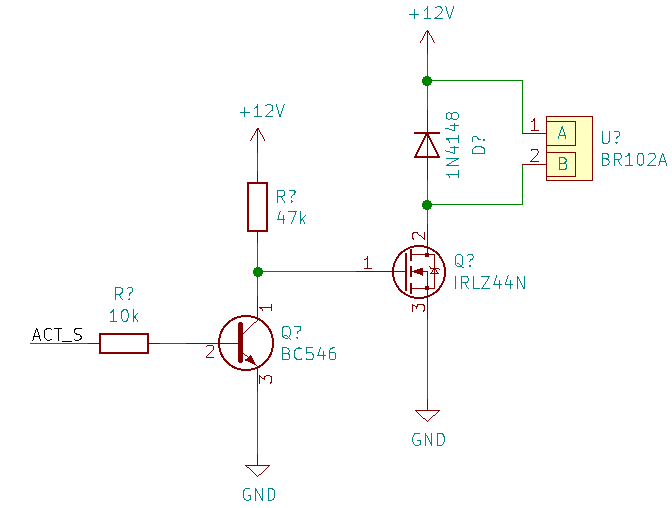
\includegraphics[width=0.5\textwidth]{figuras/ativa_valvula.png}
    \caption*{\tiny{Fonte: Própria.}}
    \label{fig:diagramavalvula}
  \end{figure} 
  
\end{frame}

\begin{frame}{Desenvolvimento dos elementos de \textit{Firmware}}{Instalação e configuração do \textit{Broker MQTT}}
  \begin{itemize}
    \item  A configuração do \textit{broker} leva em consideração quatro informações: \textbf{endereço de IP}, \textbf{porta}, \textbf{usuário} e \textbf{senha}.
  \end{itemize}
 
  \begin{block}{}
    \begin{itemize}
      \item sudo apt-get install mosquitto
      \item sudo apt-get install mosquitto-clients
      \item sudo stop mosquitto
      \item sudo mosquitto\_passwd -c /etc/mosquitto/passwd $<$user\_name$>$
    \end{itemize} 
  \end{block} 
\end{frame}

\begin{frame}{Desenvolvimento dos elementos de \textit{Firmware}}{Instalação e configuração do \textit{Broker MQTT}}
  \begin{figure}[H]
    \centering
    \caption{Arquivo de credenciais do Mosquitto gerado}
    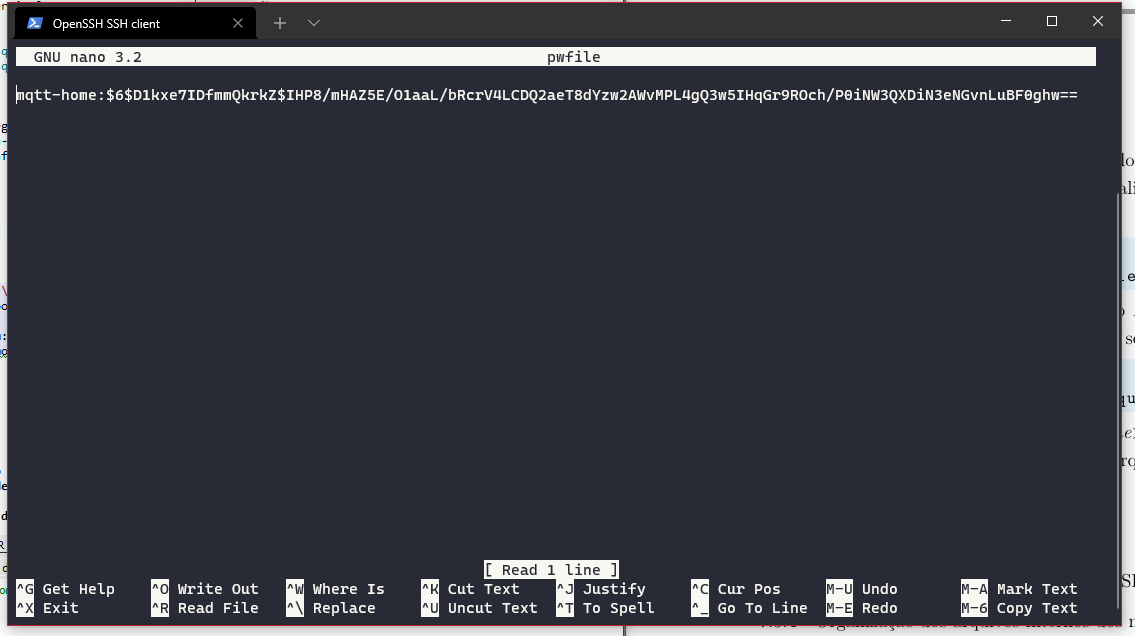
\includegraphics[width=0.6\textwidth]{figuras/user_pass.png}
    \caption*{\tiny{Fonte: Própria.}}
    \label{fig:cred_mqtt}
  \end{figure}
\end{frame}

\begin{frame}{Desenvolvimento dos elementos de \textit{Firmware}}{Instalação e configuração do \textit{Broker MQTT}}
  \begin{figure}[H]
    \centering
    \caption{Em destaque, IP estático configurado no roteador local.}
    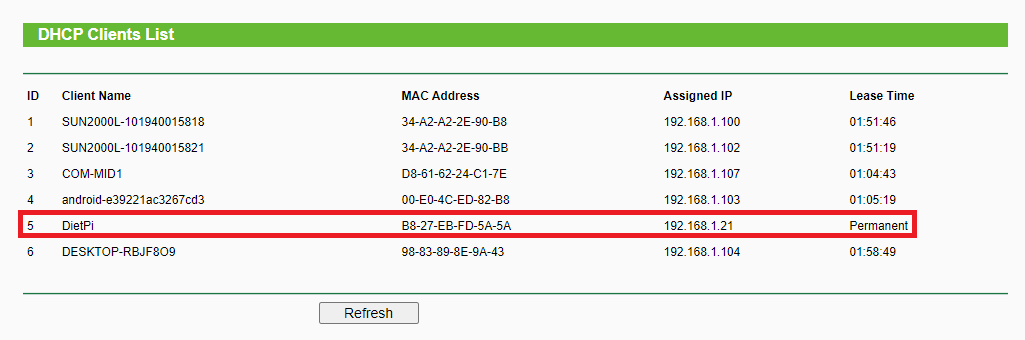
\includegraphics[width=1
    \textwidth]{figuras/ip_estatico_rasp.png}
    \caption*{\tiny{Fonte: Própria.}}
    \label{fig:roteador}
  \end{figure}
\end{frame}

\begin{frame}{Desenvolvimento dos elementos de \textit{Firmware}}{{Definição de utilização dos pinos do ESP-12S}}
  \begin{figure}[H]
    \centering
    \caption{Declarações dos pinos realizadas no código do módulo \textbf{CCM}.}
    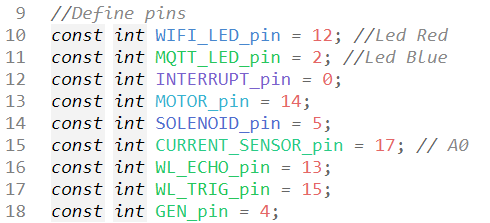
\includegraphics[width=0.5
    \textwidth]{figuras/pinos_definicao_ccm2.png}
    \caption*{\tiny{Fonte: Própria.}}
    \label{fig:definicao_pinos_ccm}
  \end{figure}
\end{frame}

\begin{frame}{Desenvolvimento dos elementos de \textit{Firmware}}{{Definição de utilização dos pinos do ESP-12S}}
  \begin{figure}[H]
    \centering
    \caption{Declarações dos pinos realizadas no código do módulo \textbf{TCM}.}
    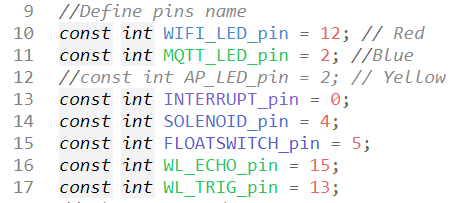
\includegraphics[width=0.5
    \textwidth]{figuras/pinos_definicao_tcm.png}
    \caption*{\tiny{Fonte: Própria.}}
    \label{fig:definicao_pinos_tcm}
  \end{figure}
\end{frame}


\begin{frame}{Desenvolvimento dos elementos de \textit{Firmware}}{Organização dos arquivos internos dos microcontroladores}

  \begin{table}[H]
    \centering
    \resizebox{\textwidth}{!}{%
      \begin{tabular}{c|c}
        \hline
        Arquivo &  Função \\ \hline
        system\_info.json &  \begin{tabular}[c]{@{}c@{}} armazena a versão do firmware, versão do sistema de arquivos,\\ data do ultimo update e o link para o repositório de novos binários \end{tabular} \\ \hline
        register\_config.json &  \begin{tabular}[c]{@{}c@{}} armazena os dados para conexão WI-FI (\textit{ssid} e senha) e os dados para conexão ao \\ \textit{broker} MQTT (IP, porta, usuário, senha, tópico de inscrição e o tópico de publicação) \end{tabular} \\ \hline
        new\_network.html & \begin{tabular}[c]{@{}c@{}} página para cadastro de do dispositivo na rede WI-FI e ao servidor MQTT \end{tabular} \\ \hline
        confirm.html & \begin{tabular}[c]{@{}c@{}} página de confirmação para recebimento dos dados após o cadastro \end{tabular}  \\ \hline
      \end{tabular}%
    }
    \caption{Descrição dos arquivos salvos na memória interna do microcontrolador.}
    \label{tab:file_system_esp}
  \end{table}
  
\end{frame}

\begin{frame}{Desenvolvimento dos elementos de \textit{Firmware}}{Comunicação com o sensor de nível}
  \begin{figure}[H]
    \centering
    \caption{Função para realizar a leitura de distância a partir do sensor ultrassônico.}
    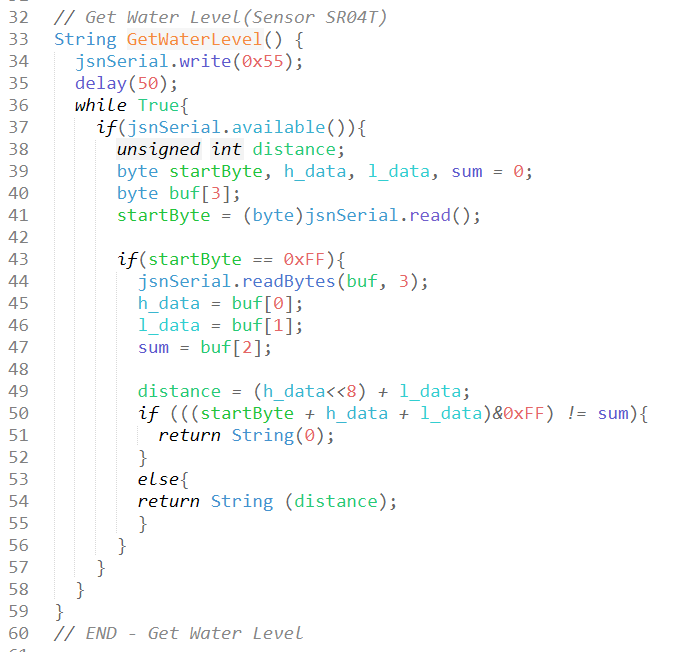
\includegraphics[width=0.4
    \textwidth]{figuras/get_water_level.png}
    \caption*{\tiny{Fonte: Própria.}}
    \label{fig:code_jsn-sr04t}
  \end{figure}
\end{frame}

\begin{frame}{Desenvolvimento dos elementos de \textit{Firmware}}{Implementação do \textit{Driver WI-FI}}
  \begin{itemize}
    \item Um módulo, seja ele um \textbf{TCM} ou \textbf{CCM}, na sua primeira utilização será necessário configurar: a rede \textit{WI-FI} para se conectar, o servidor \textit{broker} e os tópicos de inscrição e de publicação;
  \end{itemize}
  
\end{frame}

\begin{frame}{}
  \vspace*{-0.3cm}
  \begin{figure}[H]
    \centering
    \caption{Diagrama de operação do microcontrolador.}
    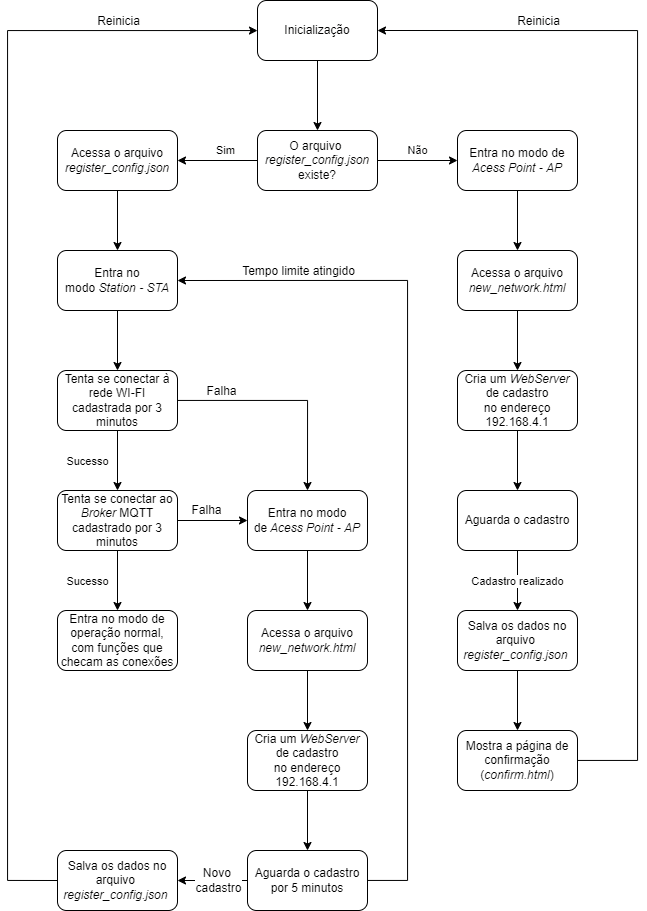
\includegraphics[width=0.47\textwidth]{figuras/firmware_sequence.png}
    \vspace*{-0.1cm}
    \caption*{\tiny{Fonte: Própria.}}
    \label{fig:firmware_sequence}
  \end{figure}
\end{frame}

\begin{frame}{Desenvolvimento dos elementos de \textit{Firmware}}{Implementação do \textit{Driver WI-FI}}
  \begin{figure}[H]
    \centering
    \caption{Página \textit{HTML} gerada para cadastro do dispositivo.}
    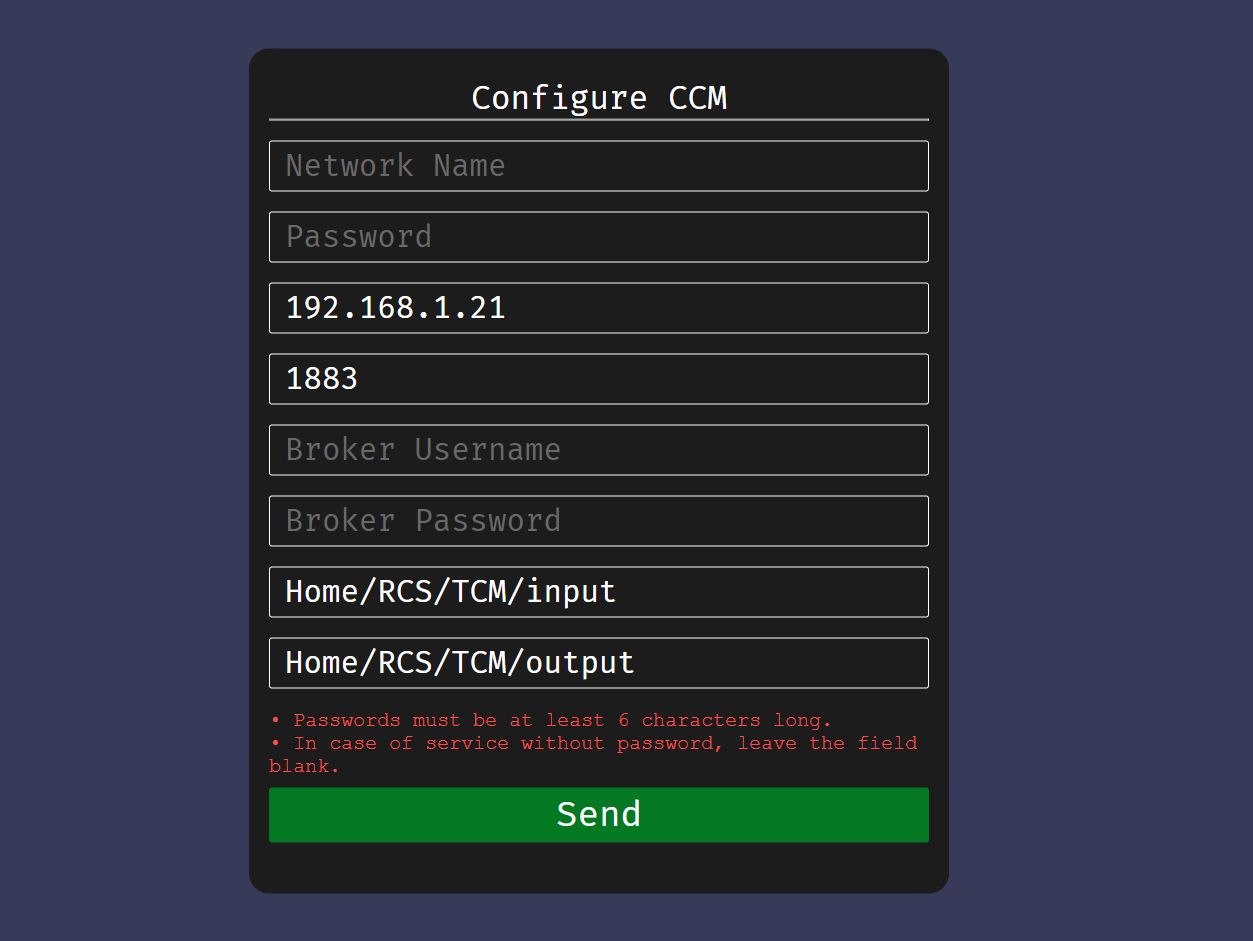
\includegraphics[width=0.6\textwidth]{figuras/cadastro_client.png}
    \caption*{\tiny{Fonte: Própria.}}
  \end{figure}
\end{frame}

\begin{frame}{Desenvolvimento dos elementos de \textit{Firmware}}{Implementação do \textit{Driver MQTT}}
  \begin{figure}[H]
    \centering
    \caption{Função de \textit{Callback}.}
    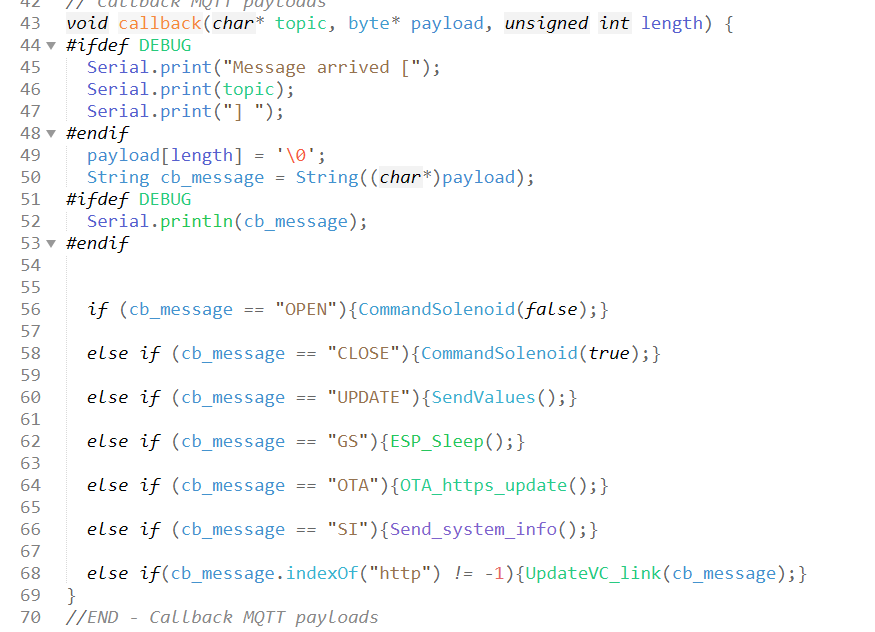
\includegraphics[width=0.6\textwidth]{figuras/drive_mqtt.png}
    \caption*{\tiny{Fonte: Própria.}}
    \label{fig:drive_mqtt}
  \end{figure}
\end{frame}

\begin{frame}{Desenvolvimento dos elementos de \textit{Firmware}}{Implementação do \textit{Driver MQTT}}
  \begin{table}[H]
    \centering
    \resizebox{12cm}{!}{
      \begin{tabular}{c|c}
        \hline
        Menssagem     & Ação                                                  \\ \hline
        ON          & Liga a motobomba                                      \\ \hline
        OFF         & Desliga a motobomba                                   \\ \hline
        OPEN        & Abre a válvula solenoide                              \\ \hline
        CLOSE       & Fecha a válvula solenoide                             \\ \hline
        UPDATE      & Retorna um arquivo json com os dados sesores          \\ \hline
        GS          & Coloca o processador em modo de DeepSleep             \\ \hline
        OTA         & Verifica se há uma atualização de firmware disponível \\ \hline
        SI          & Retorna o um arquivo json com os dados do sistema     \\ \hline
        HTTP + LINK & Cadastra um novo link para busca de atualizações      \\ \hline
      \end{tabular}%
    }
    \caption{Comandos válidos para os módulos TCM e CCM}
    \label{tab:mqtt_commands}
  \end{table}
\end{frame}

\begin{frame}{Desenvolvimento dos elementos de \textit{Firmware}}{Implementação do \textit{Factory Reset}}
  \begin{figure}[H]
    \centering
    \caption{Função de interrupção.}
    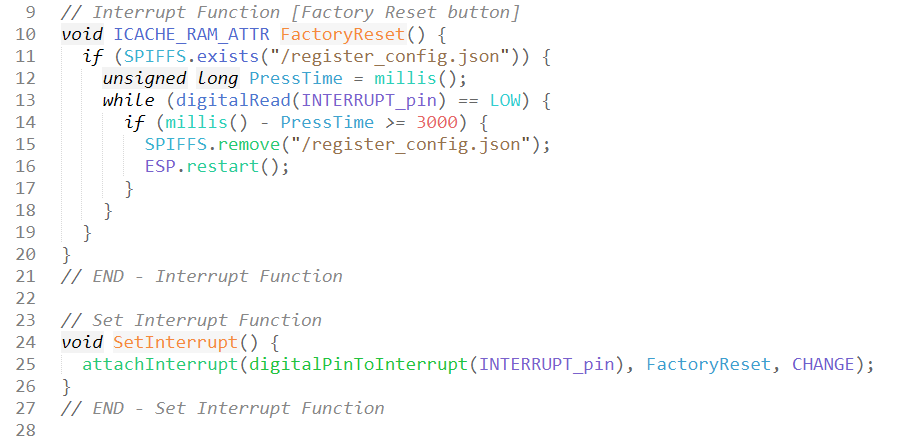
\includegraphics[width=0.8\textwidth]{figuras/interrupcao.png}
    \caption*{\tiny{Fonte: Própria.}}
    \label{fig:interrupcao}
  \end{figure}
\end{frame}

\begin{frame}{Desenvolvimento dos elementos de \textit{Firmware}}{Implementação do \textit{Factory Reset}}
  \begin{itemize}
    \item CHANGE – Interrupção é disparada quando o pino muda de estado;
    \item FALLING – Interrupção é disparada quando o pino vai do estado HIGH para LOW;
    \item HIGH – Interrupção é disparada quando o pino está no nível HIGH;
    \item LOW – Interrupção é disparada quando o pino está no nível LOW;
    \item RISING – Interrupção é disparada quando o pino vai do estado LOW para HIGH.
  \end{itemize}
\end{frame}

\begin{frame}{Desenvolvimento dos elementos de \textit{Firmware}}{Implementação da funcionalidade de \textit{OTA Upgrade}}
  \begin{figure}[H]
    \centering
    \caption{Binário gerado ao realizar o \textit{build} do código.}
    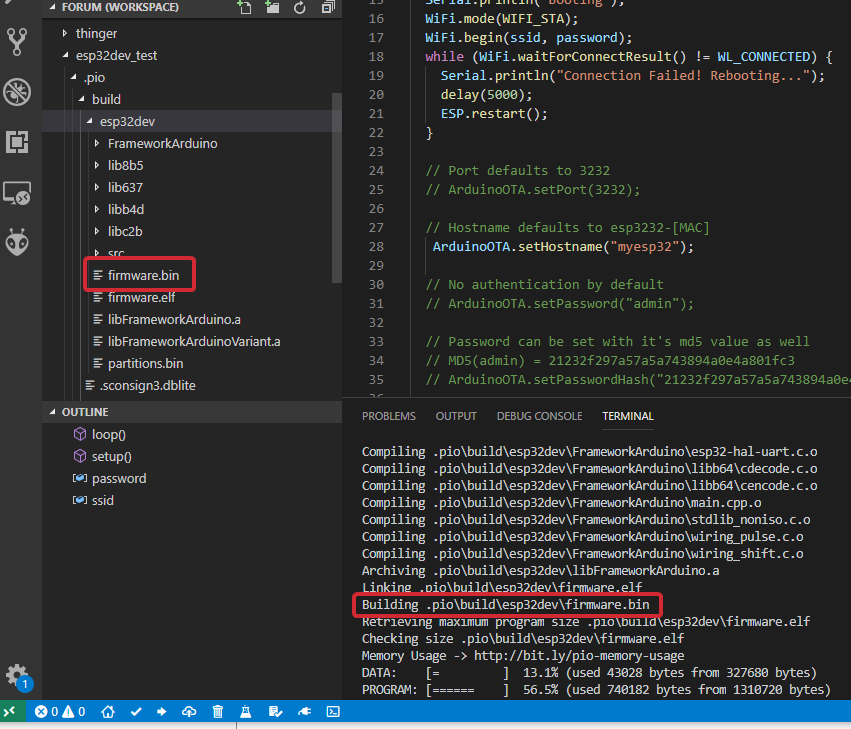
\includegraphics[width=0.5\textwidth]{figuras/platformio_bin.png}
    \caption*{\tiny{Fonte: Própria.}}
    \label{fig:bin}
  \end{figure}
  
\end{frame}

\begin{frame}{Desenvolvimento dos elementos de \textit{Firmware}}{Implementação da funcionalidade de \textit{OTA Upgrade}}
  \begin{figure}[H]
    \centering
    \caption{Repositório criado.}
    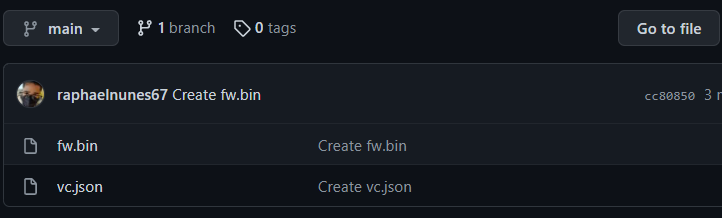
\includegraphics[width=0.6\textwidth]{figuras/repositorio_bin.png}
    \caption*{\tiny{Fonte: Própria.}}
    \label{fig:reposi}
  \end{figure}
  
\end{frame}

\begin{frame}{Desenvolvimento dos elementos de \textit{Software}}
  \begin{figure}[H]
    \centering
    \caption{Definição do \textit{layout} das telas criado no Figma.}
    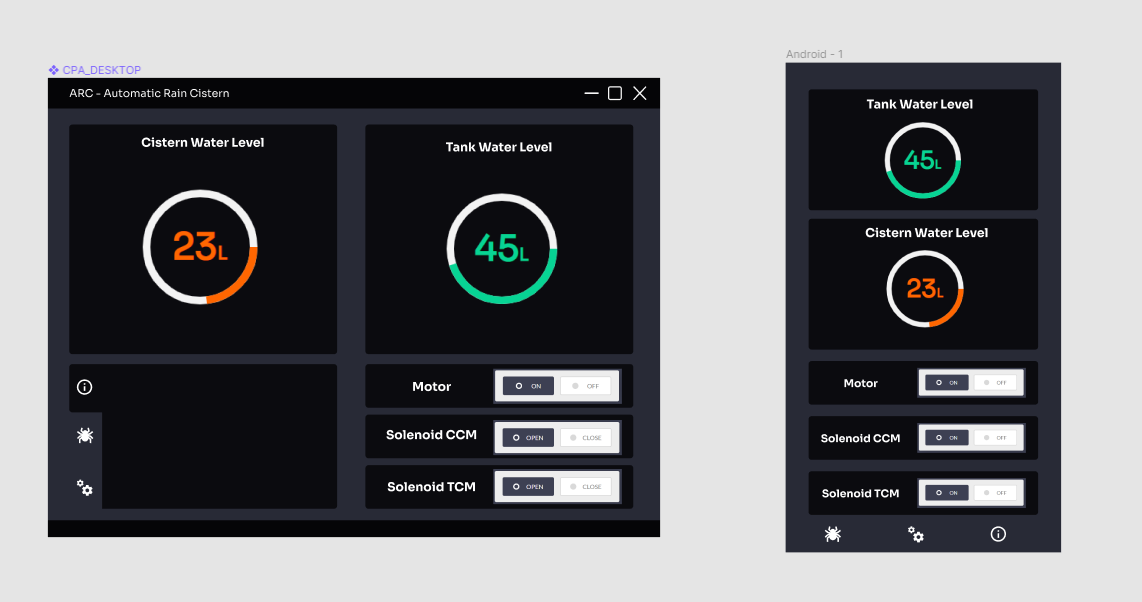
\includegraphics[width=0.6\textwidth]{figuras/figma_plan.png}
    \caption*{\tiny{Fonte: Própria.}}
    \label{fig:figma_plan_desktop}
  \end{figure}
  
\end{frame}